% ==================== 五、UML 建模 ====================
\section{UML 建模}

\subsection{图的选取与分类}

作业要求三类图各至少一张、总数不少于四张，且类图必画。本设计画了 16 张，三类都有覆盖，其中交互类多画了几张，因为本系统真正复杂的地方全在并发与异步上。

\begin{table}[H]
\centering
\caption{UML 图清单}\label{tab:uml_list}
\tabfont
\begin{tabularx}{\textwidth}{@{}L{0.6cm}L{4.5cm}L{1.6cm}X@{}}
\toprule
\# & 图名 & 类别 & 说明什么问题 \\
\midrule
1 & UML 类图 & 结构 & 领域模型 24 个类与它们的关系，是全系统数据形状的来源 \\
2 & UML 包图 & 结构 & 四层结构与十个领域包，约束依赖方向 \\
3 & UML 组件图 & 结构 & 十个模块的调用与订阅，回答「模块之间怎么协作」 \\
4 & UML 部署图 & 结构 & 应用、缓存、数据库与外部系统的物理分布 \\
5 & UML 用例图·顾客端 & 行为 & 顾客能做什么，include / extend 关系 \\
6 & UML 用例图·前台端 & 行为 & 前台的九个用例与「入住包含排房」 \\
7 & UML 用例图·店长端 & 行为 & 店长的七个用例与「改价扩展自设价」 \\
8 & UML 用例图·平台端 & 行为 & 平台地区负责人的六个用例 \\
9 & UML 状态图·订单 & 行为 & 订单六态与超时、未到店两条时间分支 \\
10 & UML 状态图·房间 & 行为 & 房间六态与维修旁路 \\
11 & UML 活动图·下单与锁库存 & 行为 & 下单链路的三个判断点与回滚 \\
12 & UML 活动图·支付回调与订单生效 & 行为 & 回调的验签、判重与状态分支 \\
13 & UML 时序图·并发抢房 & 交互 & 两单抢最后一间，谁成功谁失败 \\
14 & UML 时序图·支付回调 & 交互 & 三种订单状态下的三条落点 \\
15 & UML 时序图·改价互斥 & 交互 & 改价与下单在同一格上互斥 \\
16 & UML 时序图·超时释放与对账 & 交互 & 超时任务与每日对账两条定时链路 \\
\bottomrule
\end{tabularx}
\end{table}

包图、组件图、部署图已在第 3 章出现过，本章不重复；下面按「类图—用例图—状态图—活动图—时序图」的顺序说明其余各图。

\subsection{结构图：类图}

\begin{figure}[htbp]
\centering
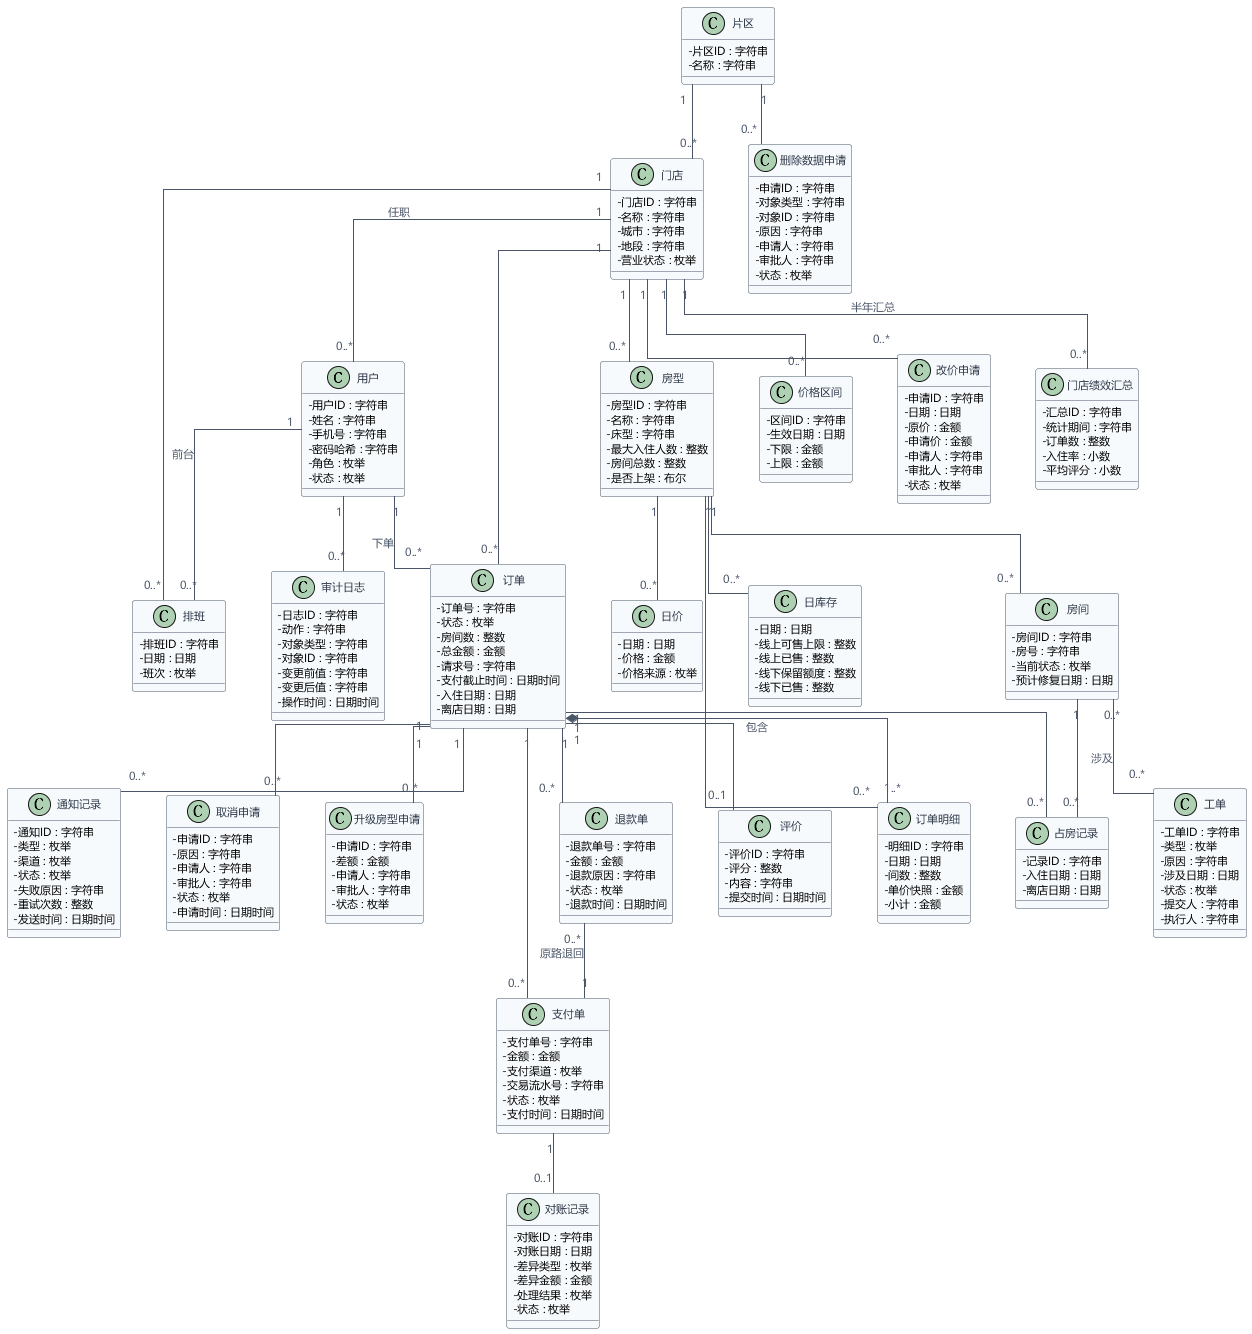
\includegraphics[width=0.94\textwidth]{../UML/UML类图.png}
\caption{UML 类图：领域模型}
\label{fig:class}
\end{figure}

类图上有 24 个类，按职责可以分成四簇：

\begin{itemize}
  \item \textbf{组织与人员}：片区、门店、用户、排班。片区 1 对多门店，门店 1 对多用户与排班。
  \item \textbf{房源与价格}：房型、房间、日价、日库存、价格区间、改价申请。房型 1 对多房间，也 1 对多日价与日库存。
  \item \textbf{交易}：订单、订单明细、支付单、退款单、取消申请、升级房型申请、占房记录。
  \item \textbf{支撑}：工单、评价、审计日志、通知记录、对账记录、删除数据申请、门店绩效汇总。
\end{itemize}

读这张图要注意三处\textbf{刻意}的连接，它们各自对应一条需求：

\textbf{一、日库存挂在房型上，不挂在房间上。} 类图里 `日库存` 与 `房型` 是一对多关系，与 `房间` 没有任何直接连线。这是 REQ-013 的直接表达：库存按房型与日期逐晚记录，下单时并不知道住哪间。

\textbf{二、订单与订单明细是组合关系，且明细上带单价快照。} `订单` 与 `订单明细` 之间是实心菱形（组合），意味着明细不能脱离订单存在；`订单明细` 有 `单价快照` 与 `小计` 两个属性，改价不回写（REQ-023）。

\textbf{三、占房记录是一个独立的关联类。} 订单与房间之间不是直接的多对多，而是通过 `占房记录` 关联，且这条记录带 `入住日期` 与 `离店日期`。原因是一间房在不同日期可以被不同订单占用，直接用多对多表达会丢掉时间维度。

还有两处容易漏的关系：`取消申请` 与 `订单` 是多对一（一张订单可能有多次取消申请，只有一条会通过），`退款单` 与 `支付单` 是多对一且注明「原路退回」（退款必须挂在原支付单上，否则不知道该退到哪个渠道）。

\subsection{行为图：四张用例图}

\begin{figure}[htbp]
\centering
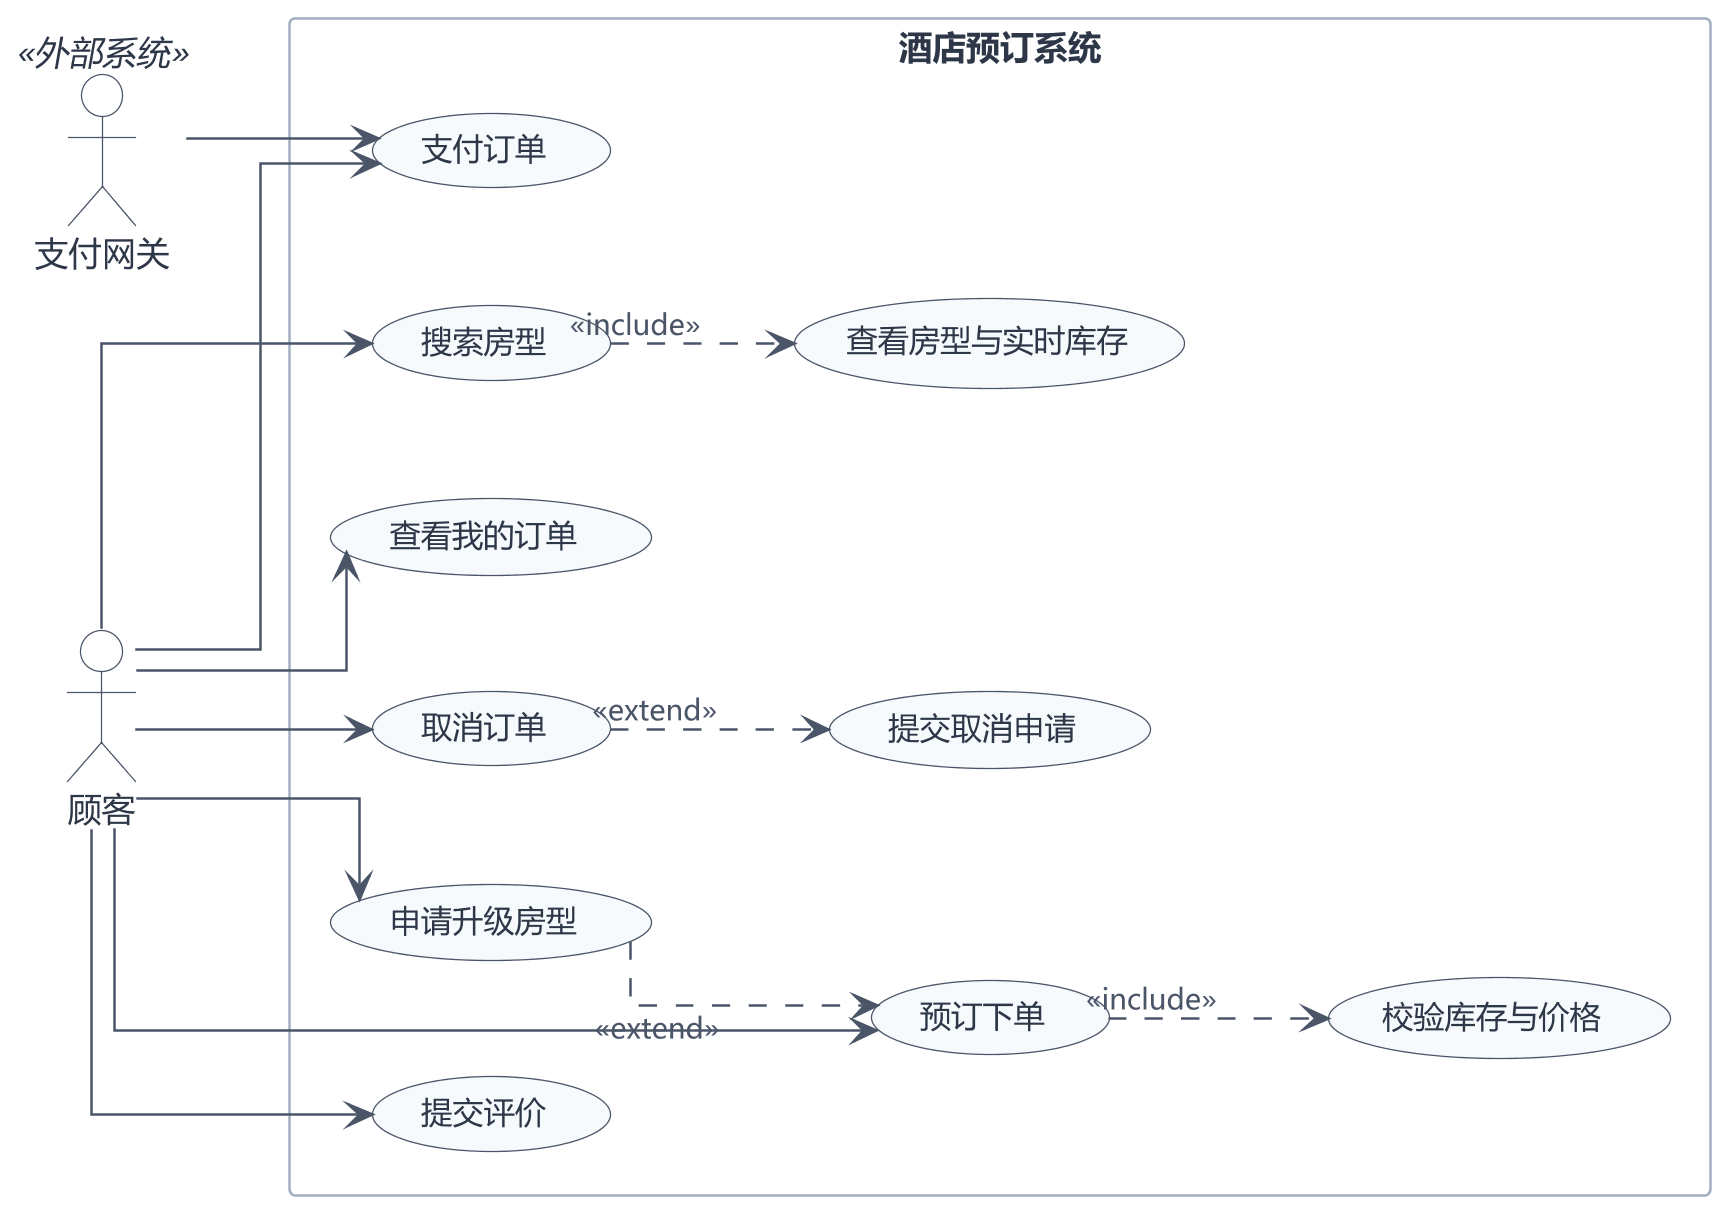
\includegraphics[width=0.86\textwidth]{../UML/UML用例图_顾客端.png}
\caption{UML 用例图：顾客端}
\label{fig:uc_c}
\end{figure}

顾客端九个用例，两条 include、两条 extend。最值得注意的是 `取消订单` 与 `提交取消申请` 是 extend 关系而不是 include——因为 18:00 之前取消根本不经过申请，只有过了 18:00 才扩展出「提交申请」这一步（REQ-021）。这一处如果画成 include，就等于说顾客每次取消都要走审批，与需求直接矛盾。

\begin{figure}[htbp]
\centering
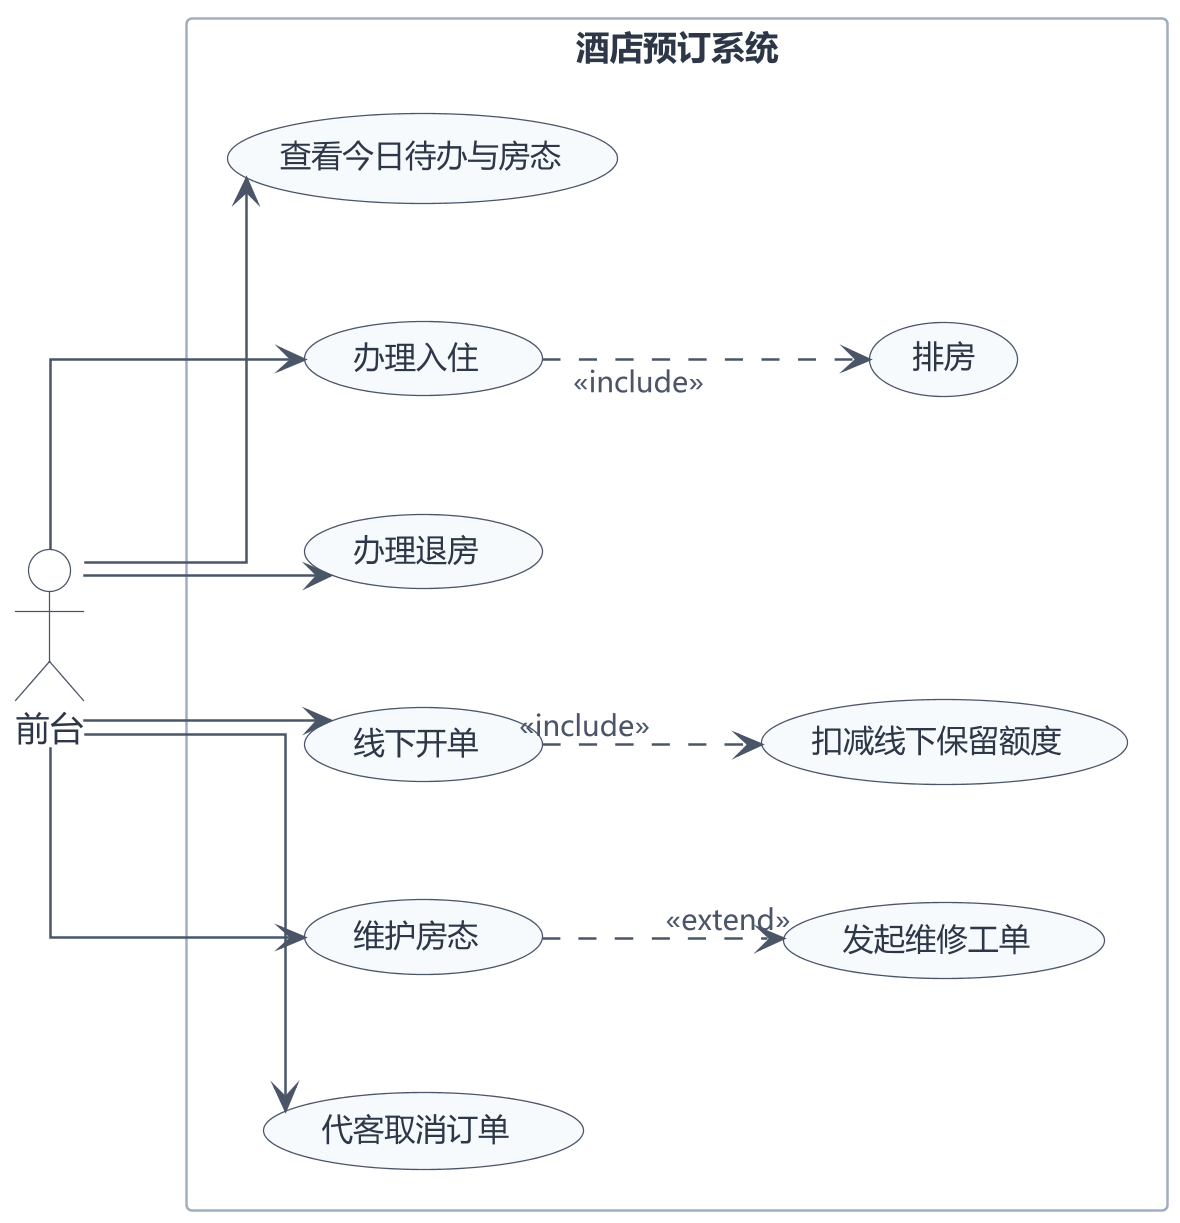
\includegraphics[width=0.86\textwidth]{../UML/UML用例图_前台端.png}
\caption{UML 用例图：前台端}
\label{fig:uc_f}
\end{figure}

前台端最关键的约束在图上是 `办理入住` include `排房`。这条 include 表达的是 REQ-018 的「3 步内完成」与 REQ-024 的「入住前必须排房」同时成立：入住一定伴随排房，但排房可以提前单独做（所以 `排房` 也是一个直接连到前台的用例）。

\begin{figure}[htbp]
\centering
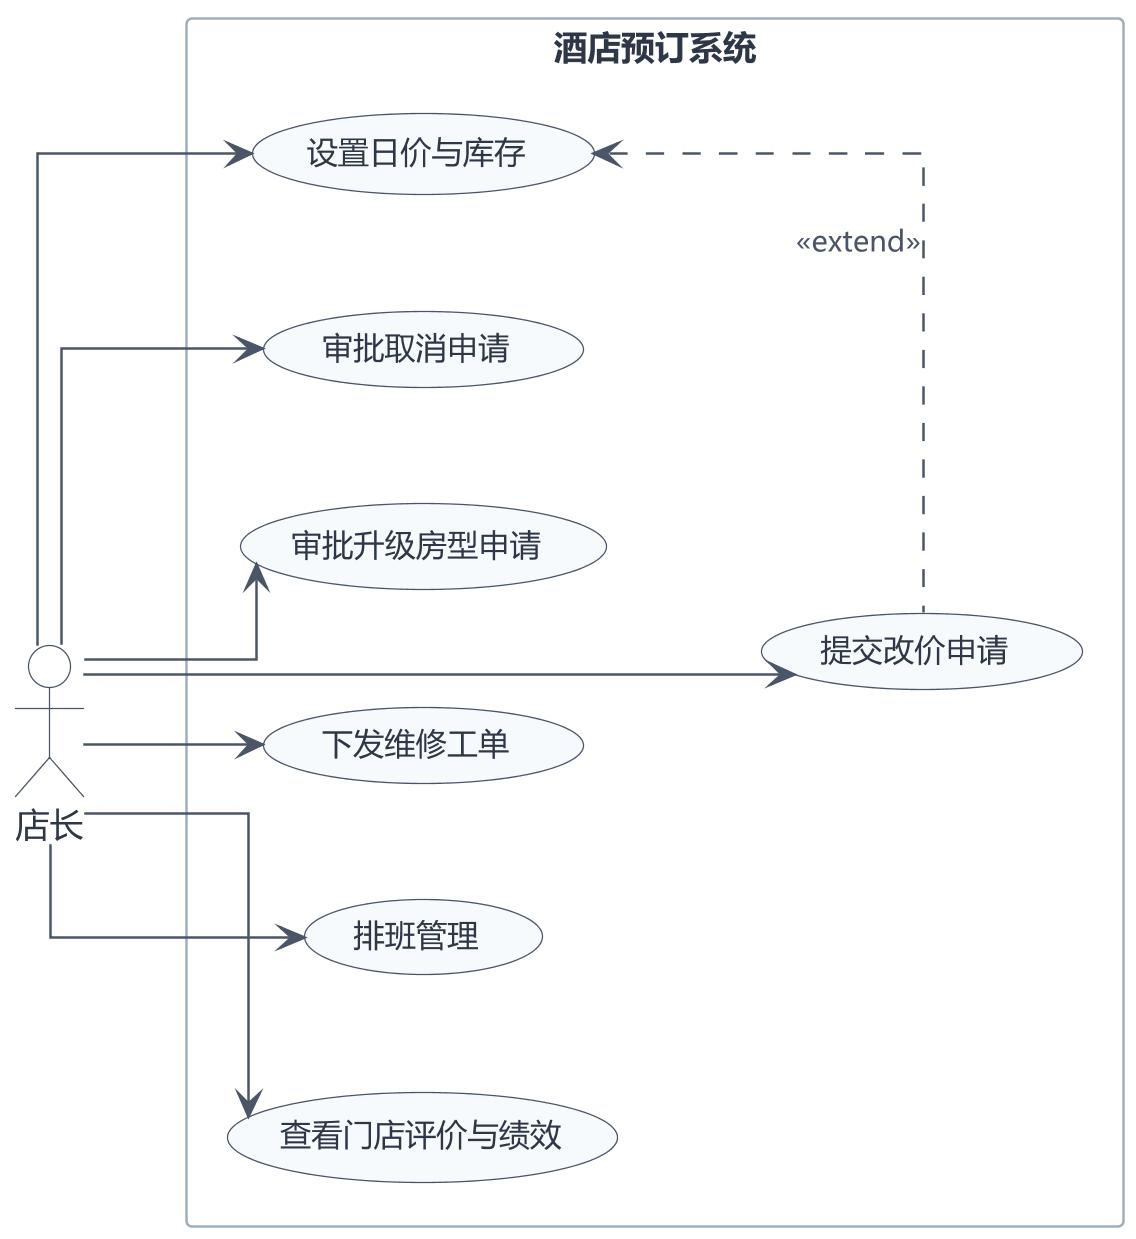
\includegraphics[width=0.8\textwidth]{../UML/UML用例图_店长端.png}
\caption{UML 用例图：店长端}
\label{fig:uc_s}
\end{figure}

店长端的 `提交改价申请` 与 `设置日价与库存` 之间是 extend：店长可以自己直接设价（在区间内），只有超区间时才扩展成「申请」再等审批。这解释了为什么店长自己发起的改价也要走审批中心——不是权限不够，而是留痕要求（REQ-014）。

\begin{figure}[htbp]
\centering
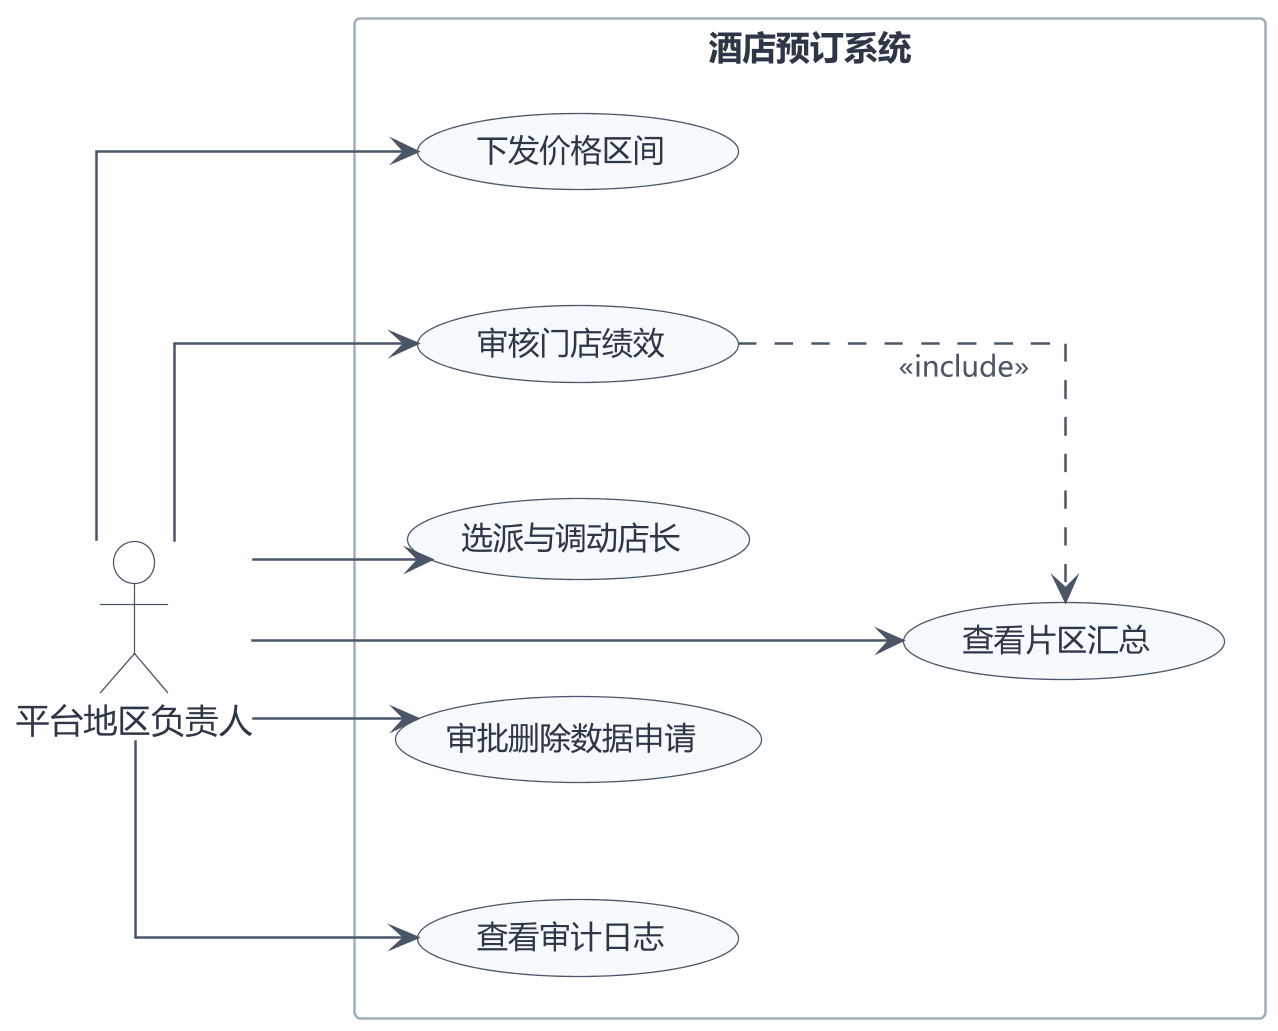
\includegraphics[width=0.8\textwidth]{../UML/UML用例图_平台端.png}
\caption{UML 用例图：平台端}
\label{fig:uc_p}
\end{figure}

平台端六个用例，`审核门店绩效` include `查看片区汇总`——审核绩效必须先看汇总，这不是可选项。图中没有「办理入住」「改房态」这类用例，是刻意的：REQ-007 明确平台地区负责人不得代门店办理业务。

\subsection{行为图：两台状态机}

\begin{figure}[htbp]
\centering
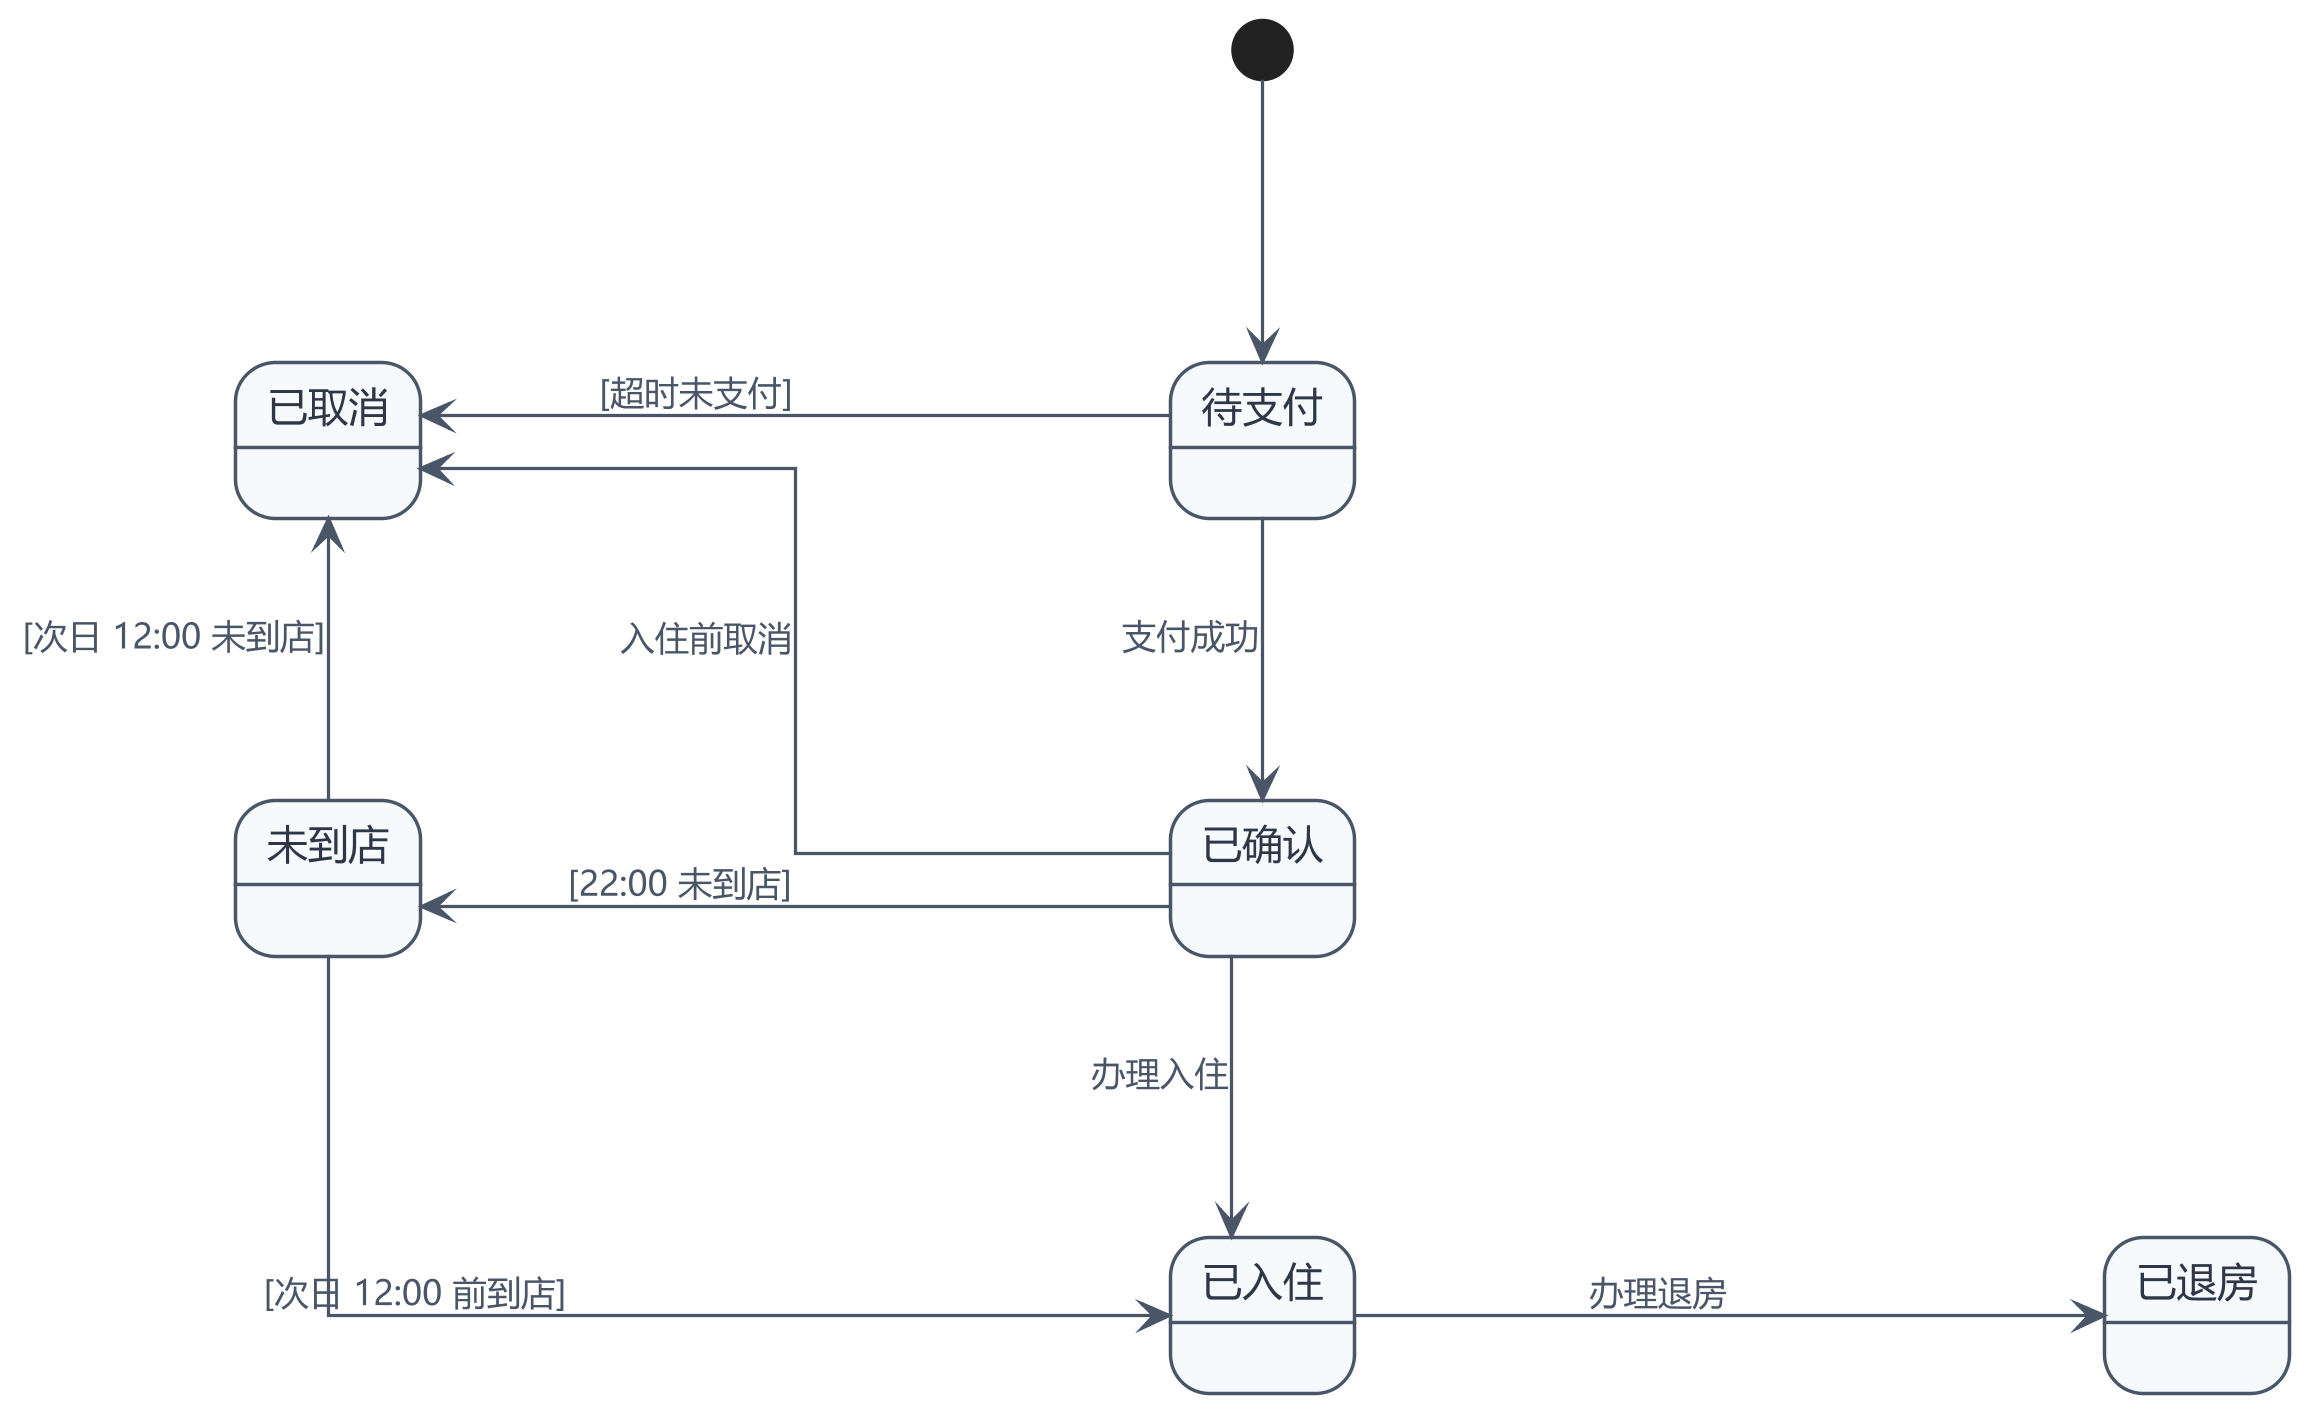
\includegraphics[width=0.82\textwidth]{../UML/UML状态图_订单.png}
\caption{UML 状态图：订单六态}
\label{fig:st_order}
\end{figure}

订单状态机的六条边里有两条带时间条件：`已确认 $\rightarrow$ 未到店` 的条件是「22:00 未到店」，`未到店 $\rightarrow$ 已取消` 的条件是「次日 12:00 仍未到店」。这两条不是业务动作触发的，是定时任务触发的，因此在状态图上用方括号条件标注，与「支付成功」「办理入住」这类动作边区分开。

对应的状态转换表如下（非法转换统一抛异常，不做「尽力修正」）：

\begin{table}[H]
\centering
\caption{订单状态转换表}
\tabfont
\begin{tabularx}{\textwidth}{@{}L{2.1cm}L{2.1cm}L{3.3cm}X@{}}
\toprule
当前状态 & 目标状态 & 触发 & 说明 \\
\midrule
（新建） & 待支付 & 顾客提交 & 同事务扣库存 \\
待支付 & 已确认 & 支付回调 & 条件更新，影响 1 行才继续 \\
待支付 & 已取消 & 超时任务 & 15 分钟未支付，同事务释放库存 \\
已确认 & 已入住 & 前台办理入住 & 与房间状态同步变更 \\
已确认 & 已取消 & 自助 / 审批通过 & 18:00 为界（REQ-021） \\
已确认 & 未到店 & 定时任务 & 入住日 22:00 \\
未到店 & 已入住 & 前台办理入住 & 仅限次日 12:00 前 \\
未到店 & 已取消 & 定时任务 & 次日 12:00，不退房费 \\
已入住 & 已退房 & 前台确认退房 & 与房间状态同步变更 \\
\midrule
\multicolumn{4}{@{}l}{\zihao{5}禁止：待支付 $\rightarrow$ 已入住 / 已退房 / 未到店；已确认 $\rightarrow$ 已退房；已入住 $\rightarrow$ 已取消 / 未到店；} \\
\multicolumn{4}{@{}l}{\zihao{5}未到店 $\rightarrow$ 已确认 / 已退房；已退房、已取消为终态；任何状态不得回到待支付。} \\
\bottomrule
\end{tabularx}
\end{table}

\begin{figure}[htbp]
\centering
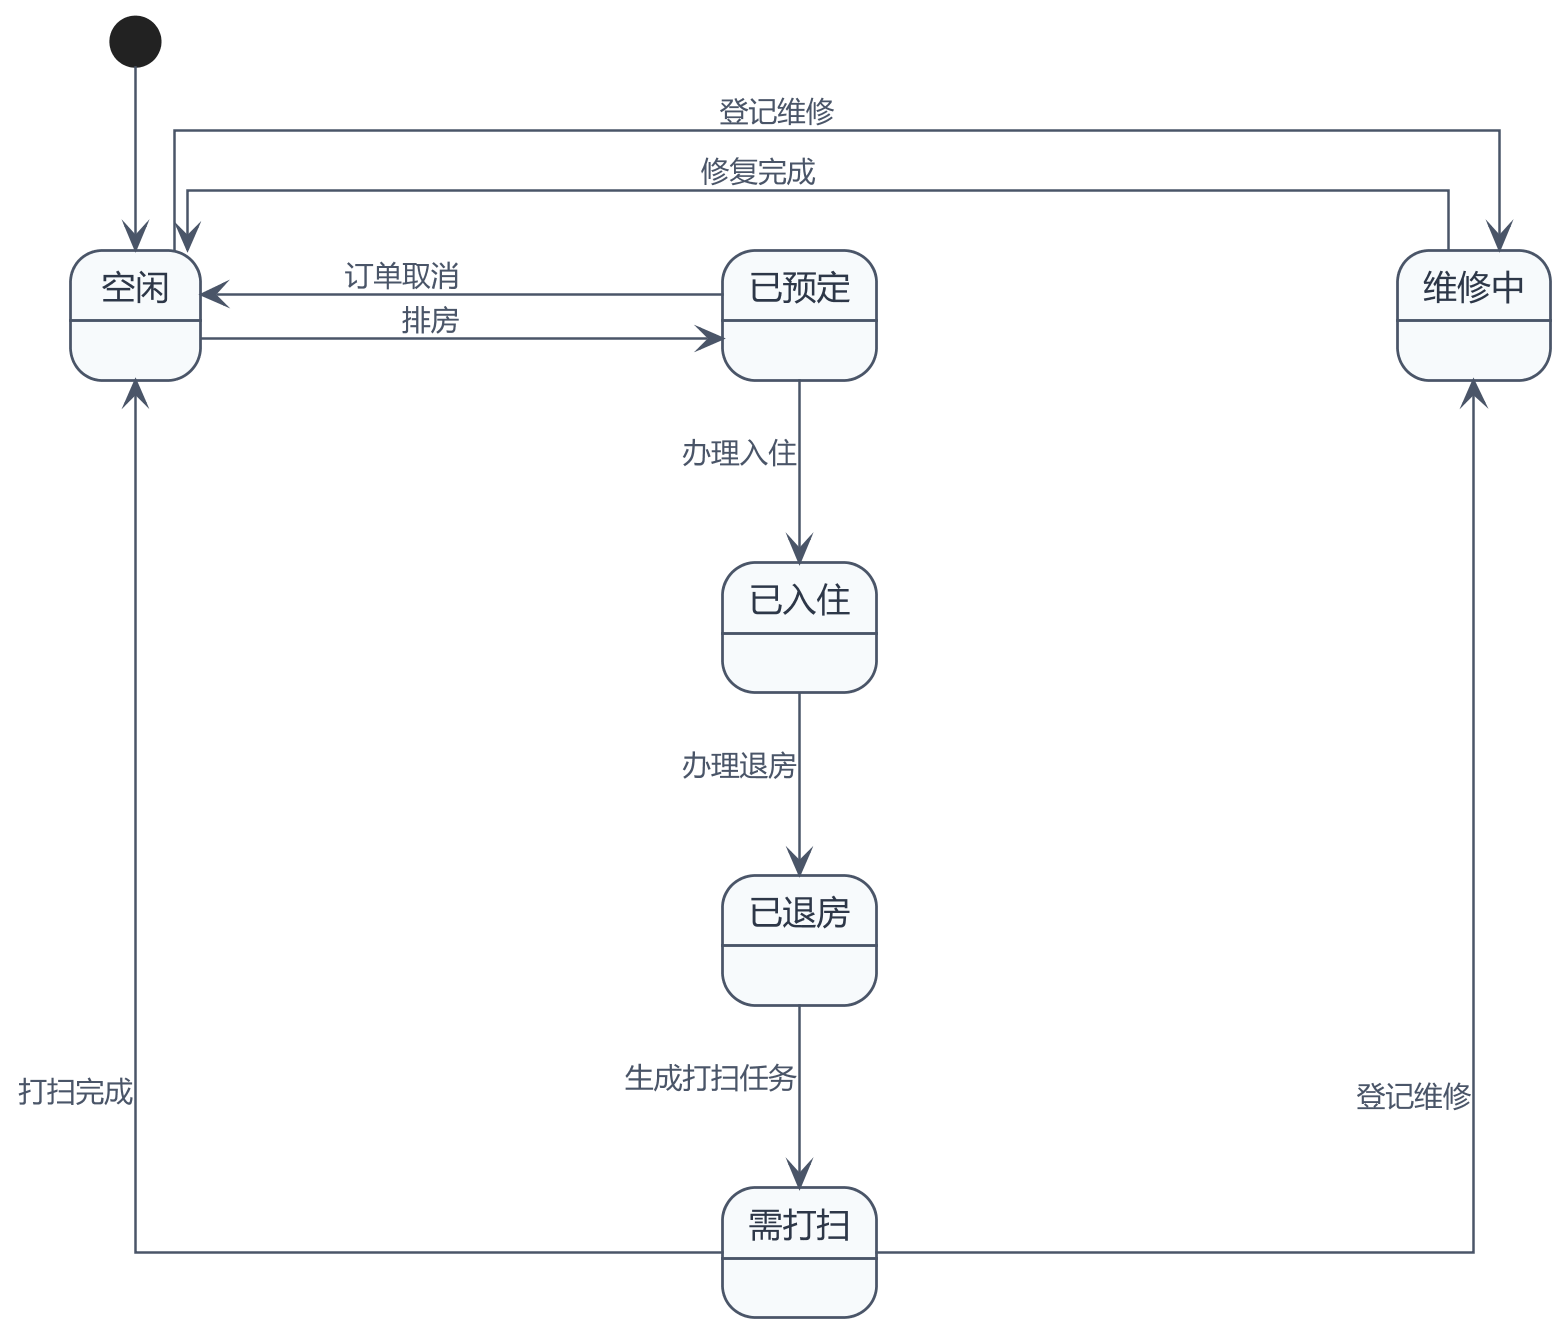
\includegraphics[width=0.78\textwidth]{../UML/UML状态图_房间.png}
\caption{UML 状态图：房间六态}
\label{fig:st_room}
\end{figure}

房间状态机比订单多一条旁路：维修中。它可以从「空闲」进入，也可以从「需打扫」进入，修复后回到「空闲」。这条旁路的意义在 REQ-034——房间转维修时，按维修日期逐日从该房型可售上限中扣除，修复当日起恢复。房态图上没有「维修中 $\rightarrow$ 已入住」这条边，是因为维修中的房间不允许排房，这一点在 REQ-024 的异常情况里写着。

\subsection{行为图：两张活动图}

\begin{figure}[htbp]
\centering
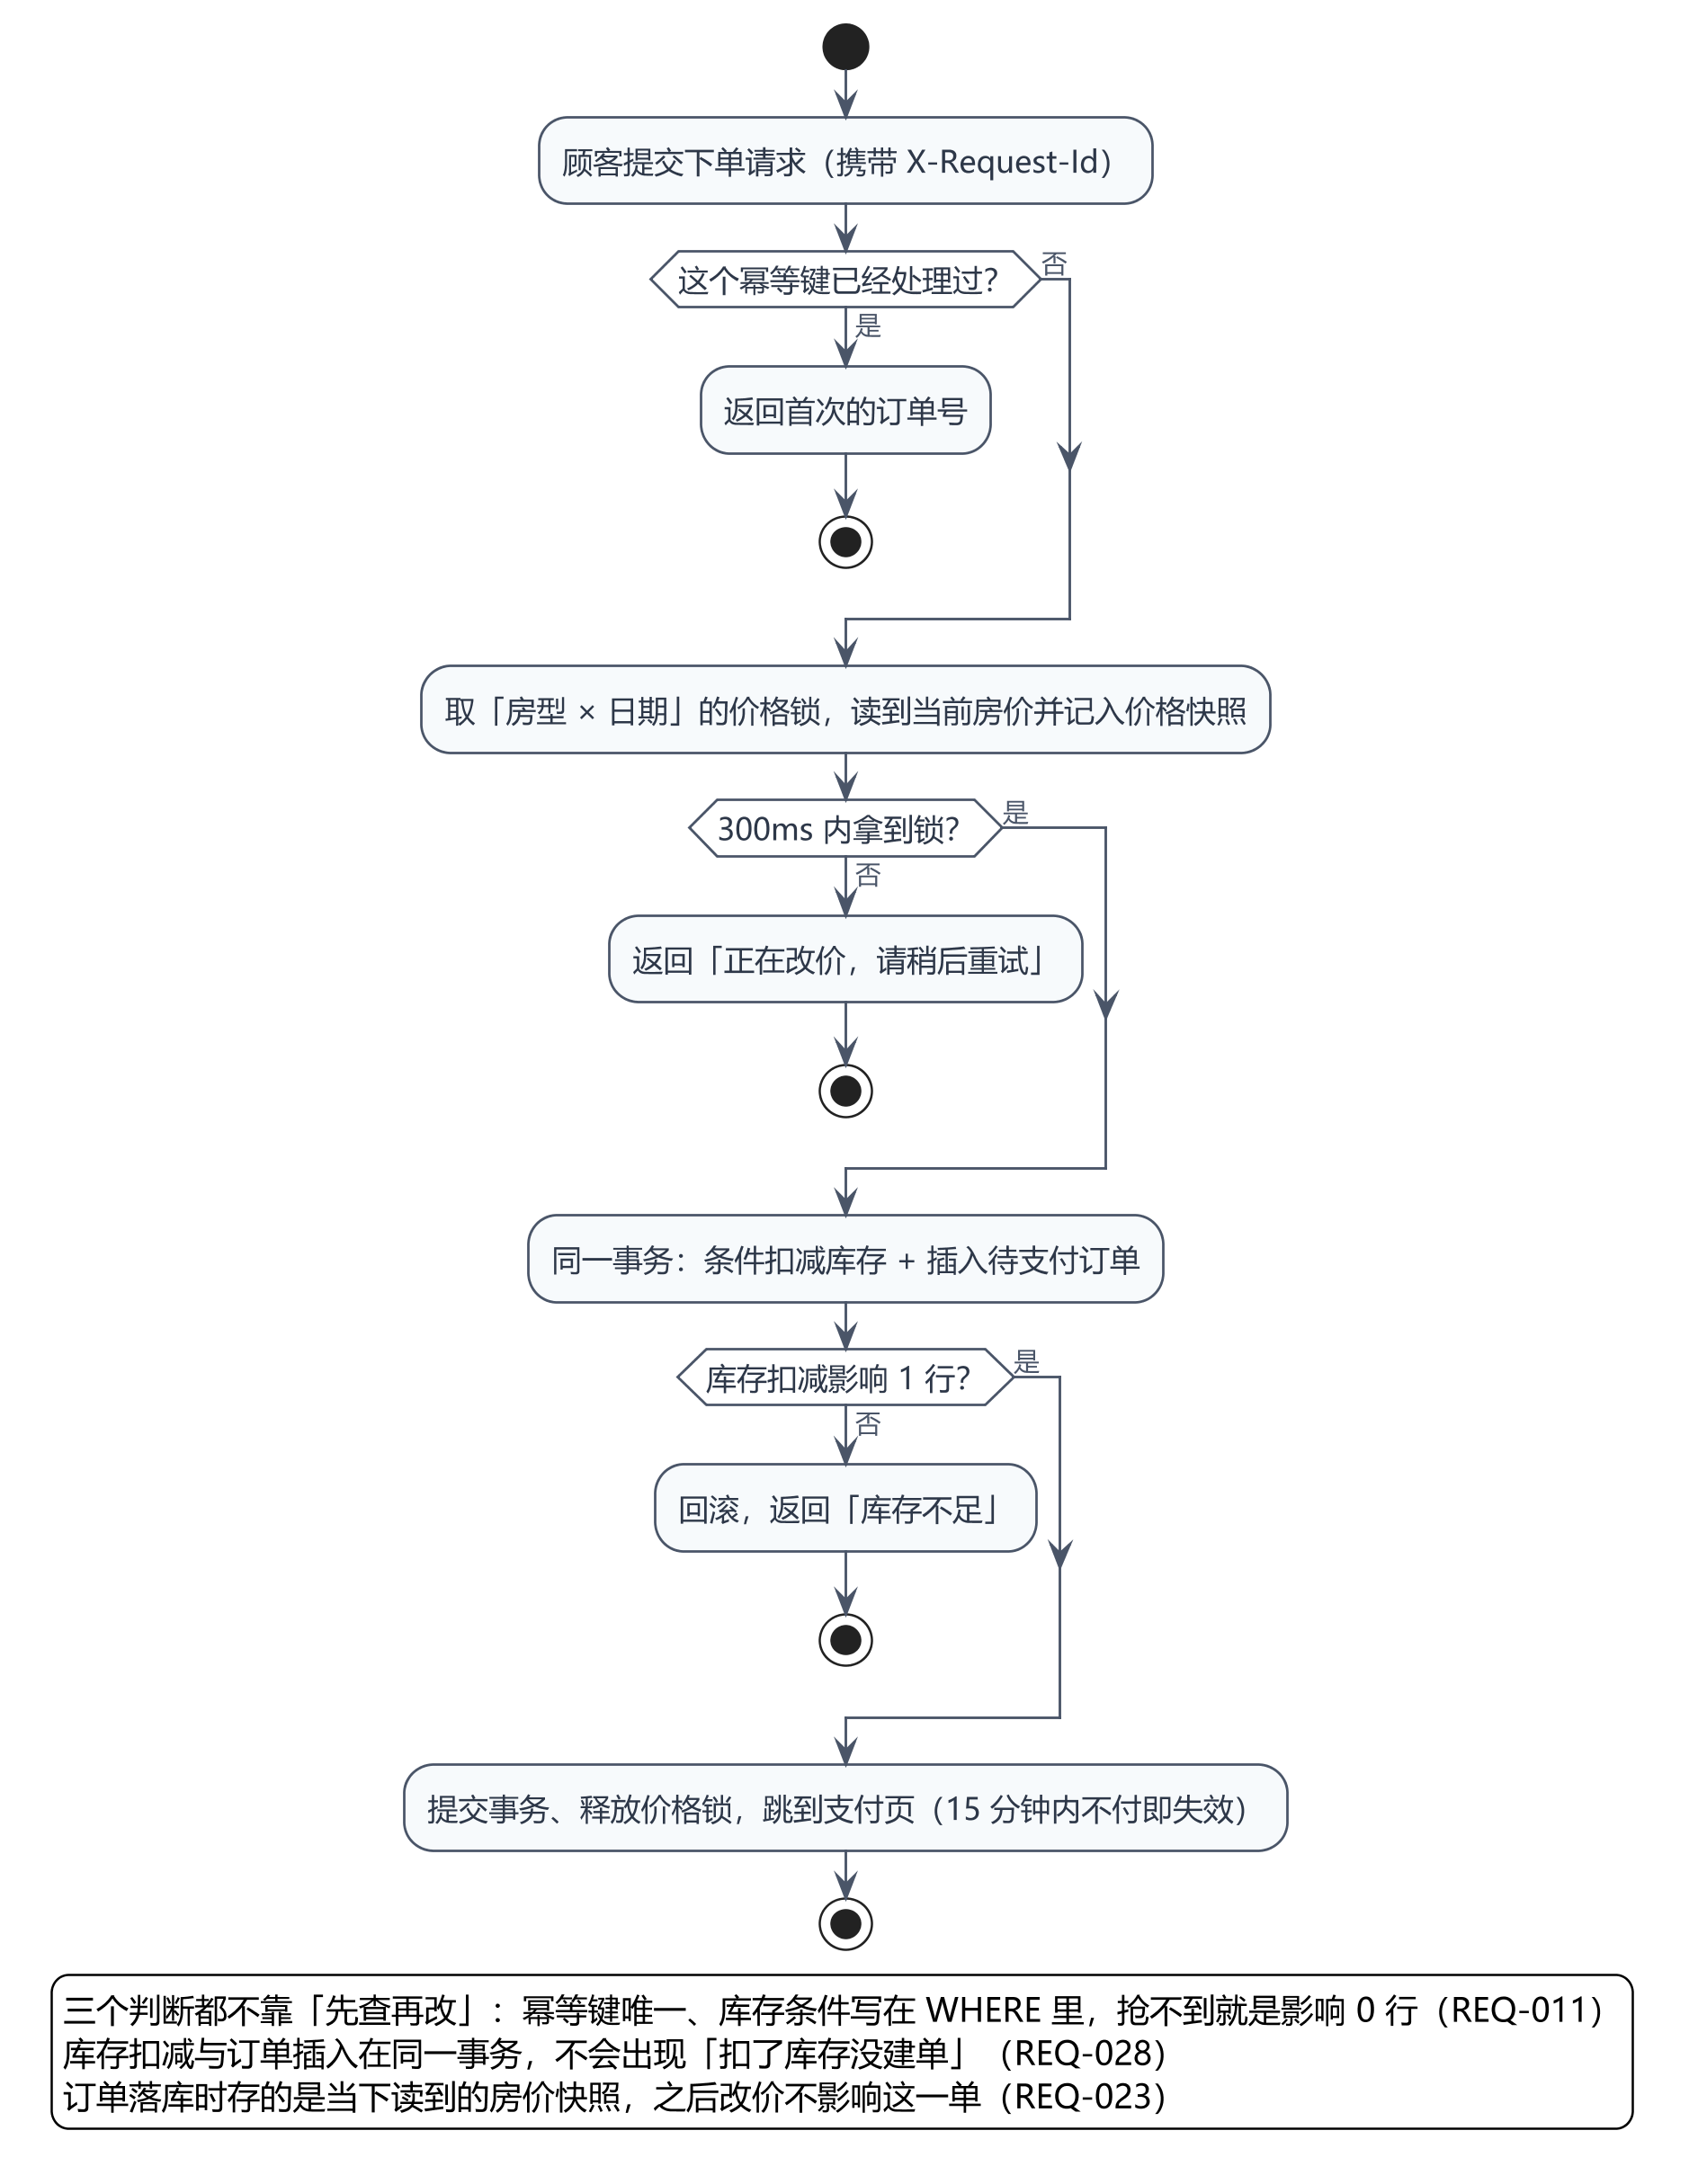
\includegraphics[width=0.62\textwidth]{../UML/UML活动图_下单与锁库存.png}
\caption{UML 活动图：下单与锁库存}
\label{fig:act1}
\end{figure}

下单活动图上有三个菱形判断，每一个都对应一种「不这么写就会出事」的场景：

\begin{enumerate}[leftmargin=3.2em]
  \item \textbf{幂等键是否已经处理过？} 是则直接返回首次的订单号，不新建订单（REQ-010）。
  \item \textbf{300 ms 内拿到价格锁了吗？} 否则返回「正在改价，请稍后重试」，\textbf{不静默用旧价}（REQ-012）。
  \item \textbf{库存条件扣减影响 1 行了吗？} 否则回滚并返回库存不足，不落任何订单（REQ-011）。
\end{enumerate}

三个判断的共同设计取向是：\textbf{失败要显式失败，不能退化成「差不多成功」}。把锁超时退化成用旧价、把库存不足退化成排队重试，都会在事后变成「订单金额不对」或「到店无房」这类无法解释的问题。

% 在进入本节前清空浮动队列，否则后续四张时序图会被推到一起、与说明文字脱节
\clearpage
\begin{figure}[htbp]
\centering
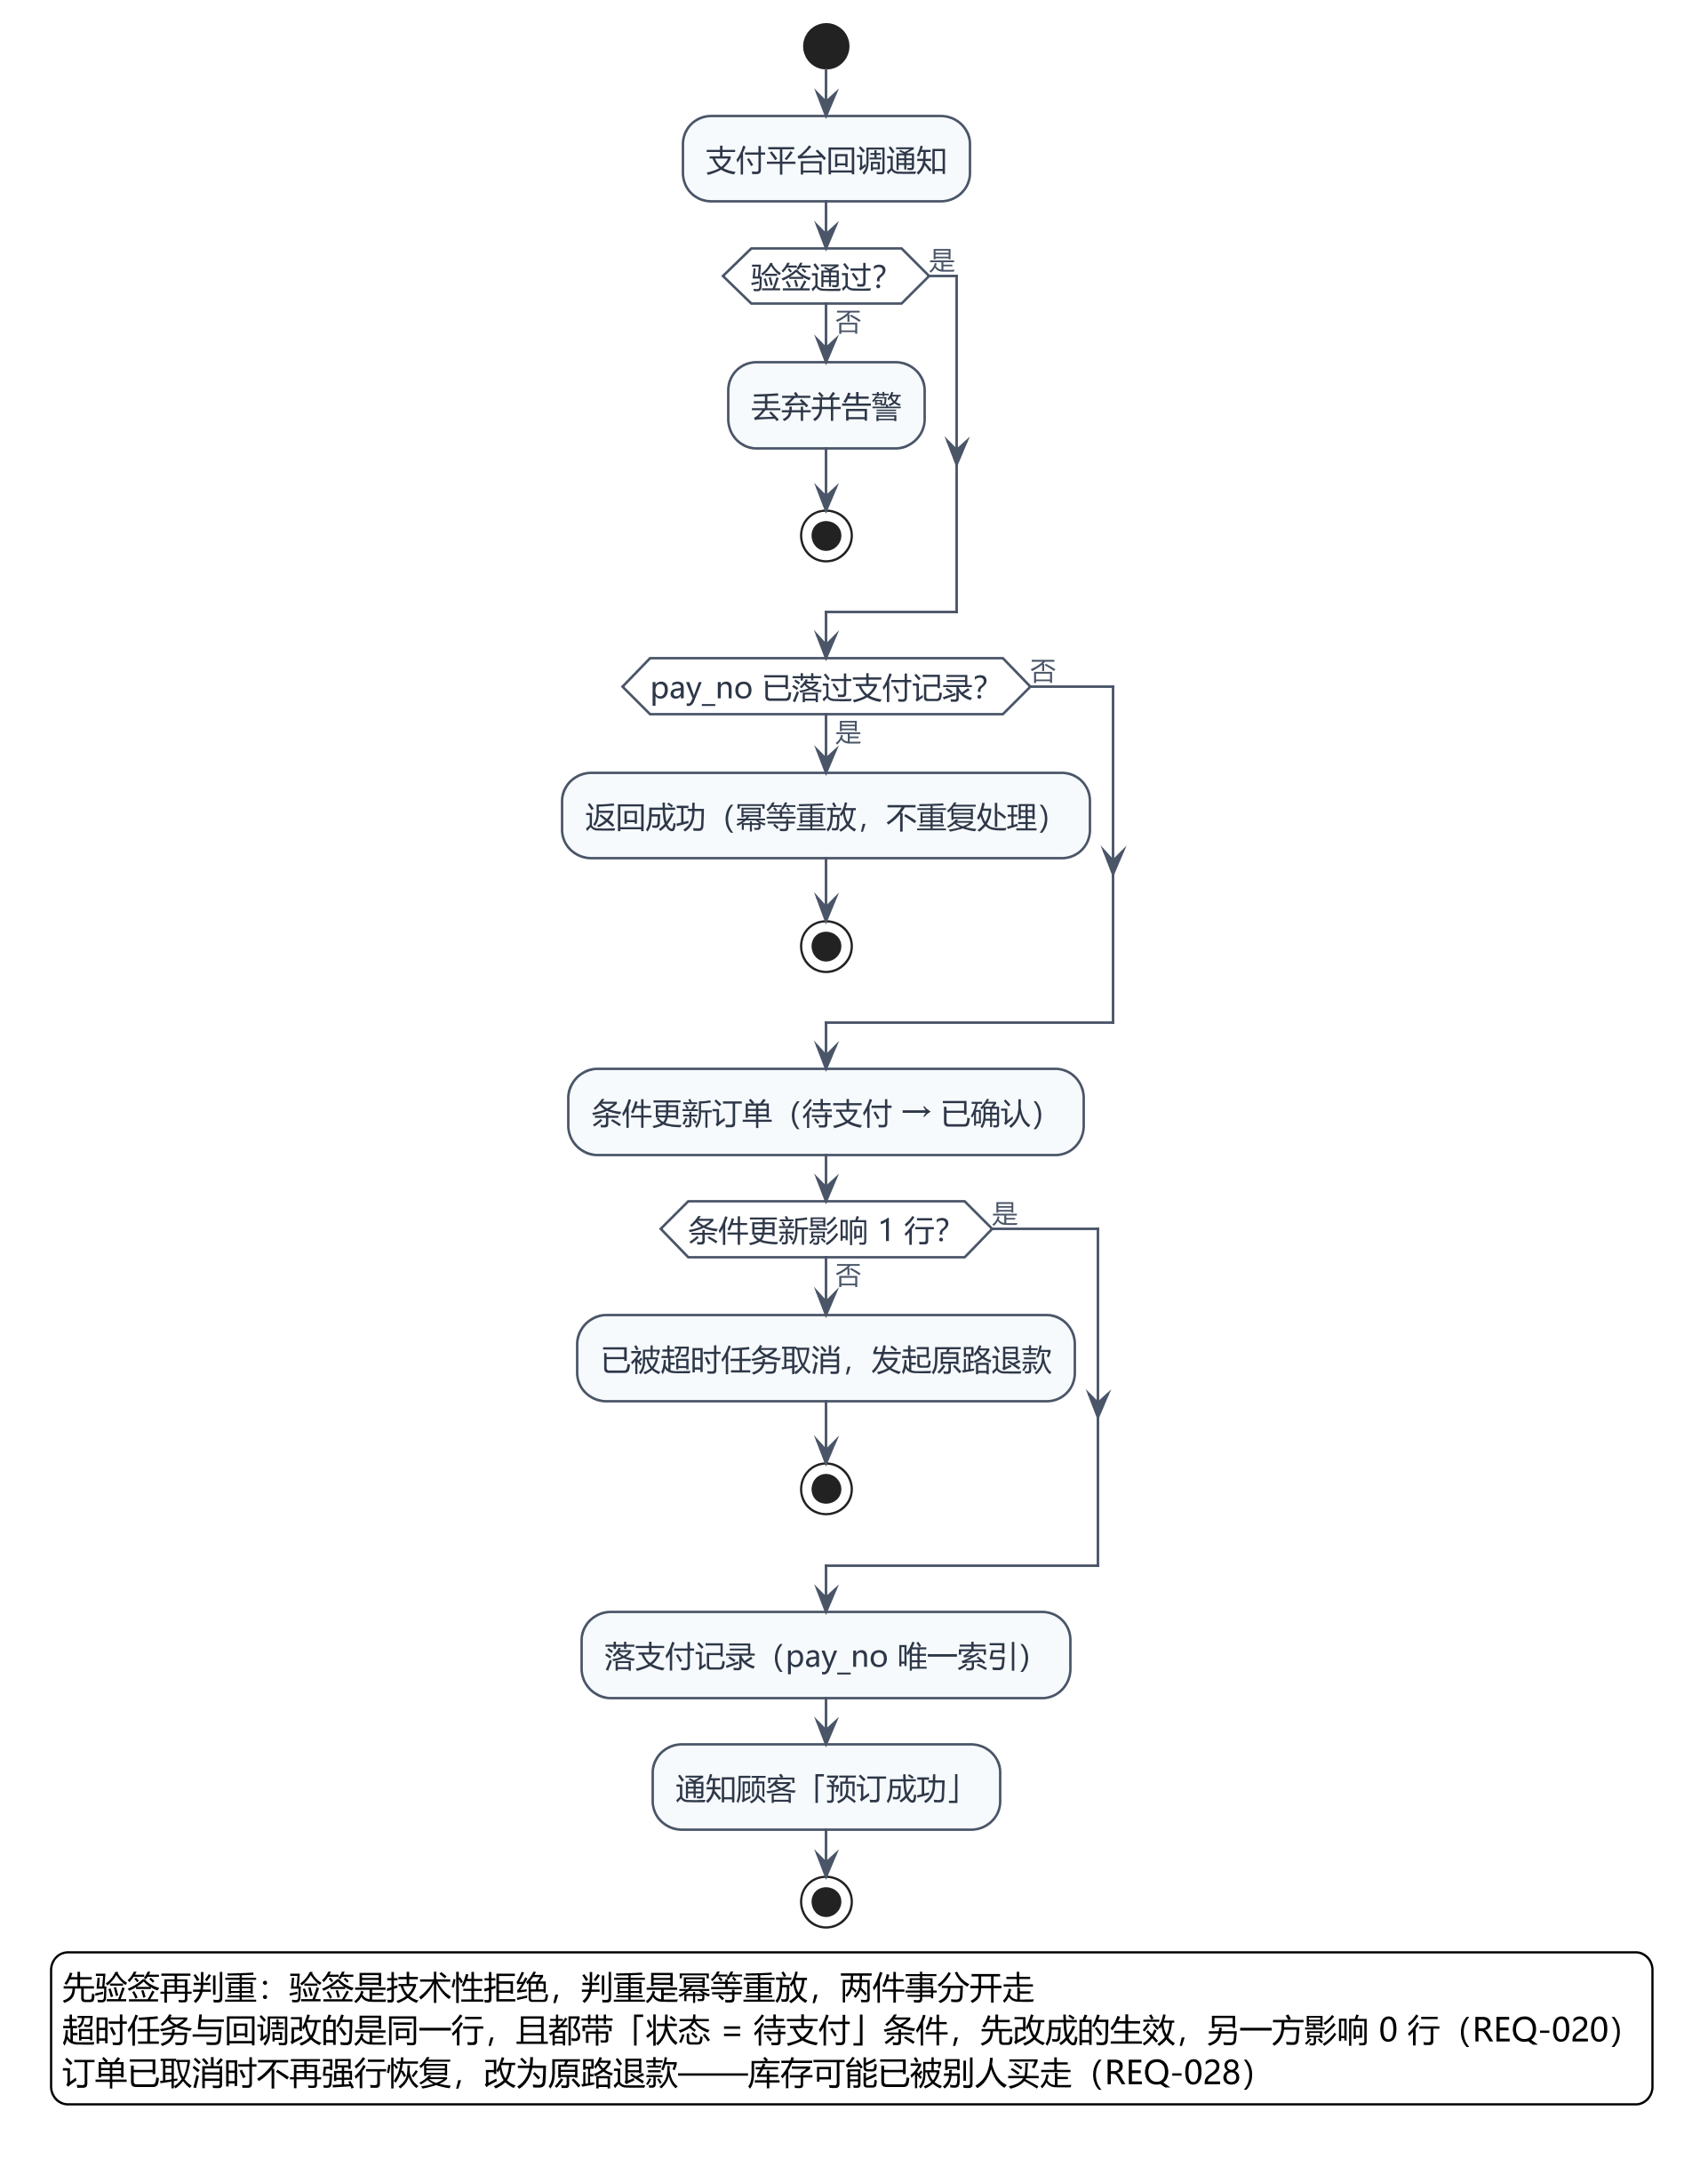
\includegraphics[width=0.62\textwidth]{../UML/UML活动图_支付回调与订单生效.png}
\caption{UML 活动图：支付回调与订单生效}
\label{fig:act2}
\end{figure}

支付回调活动图上的判断顺序是有讲究的：\textbf{先验签，再判重，最后看订单状态}。验签失败是技术性拒绝（可能是伪造请求），判重命中是正常的幂等重放（支付平台会重发），两者的日志级别、告警策略、返回码都不同，因此不能合并成一个判断。最后一步按订单\textbf{此刻}的状态分叉——已成已取消就退款而不是恢复订单，这是 REQ-028 的核心。

\subsection{交互图：四张时序图}

\begin{figure}[htbp]
\centering
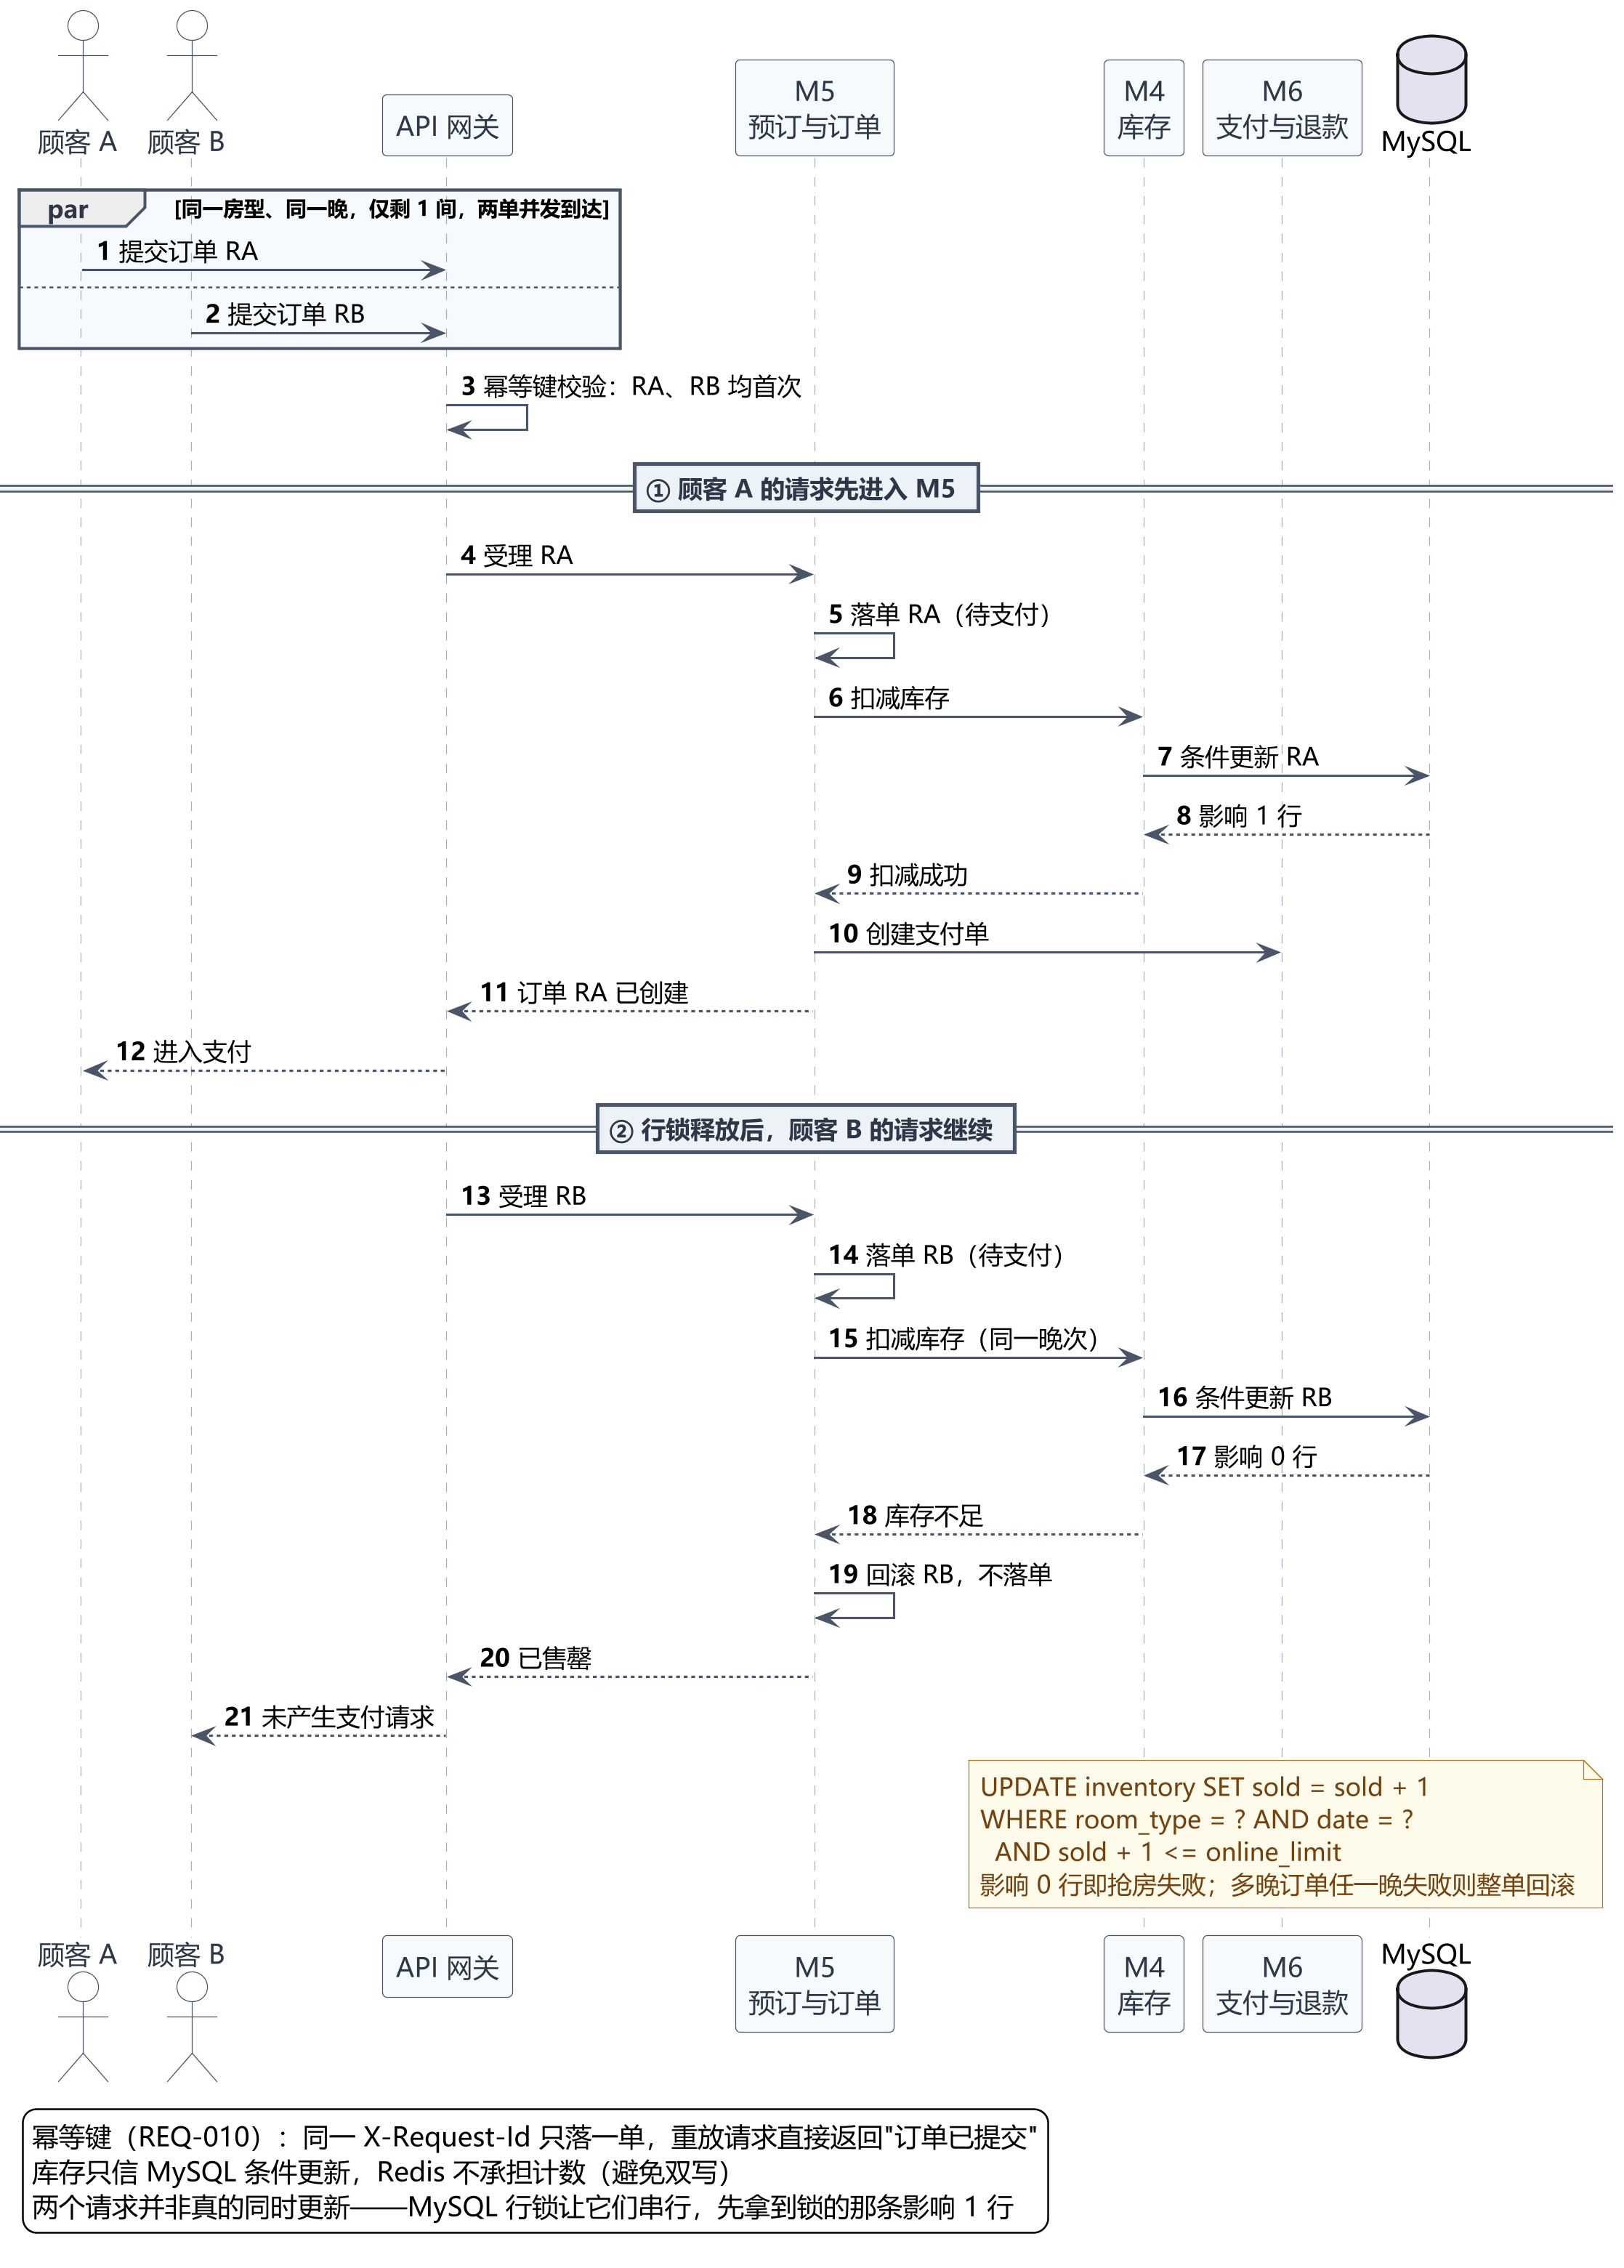
\includegraphics[width=0.68\textwidth]{../UML/UML时序图_并发抢房.png}
\caption{UML 时序图：并发抢房}
\label{fig:seq1}
\end{figure}

这张图想说明的是：所谓「并发」，在数据库层面其实是串行的。顾客 A 与 B 的请求同时到达，但两次 UPDATE 之间隔着 MySQL 的行锁，先拿到锁的那条影响 1 行，后一条影响 0 行。因此「按服务端收到提交的时间排序，最先成功者获得库存」（REQ-011）不需要额外的排序逻辑，行锁的获取顺序就是实际顺序。

同时这张图上还有一条容易忽略的线：顾客 B 抢房失败后\textbf{不产生支付请求}。这是需求里明写的边界——抢房失败却生成了支付单，就会出现「付了钱但没有房」的对账差异。

\begin{figure}[htbp]
\centering
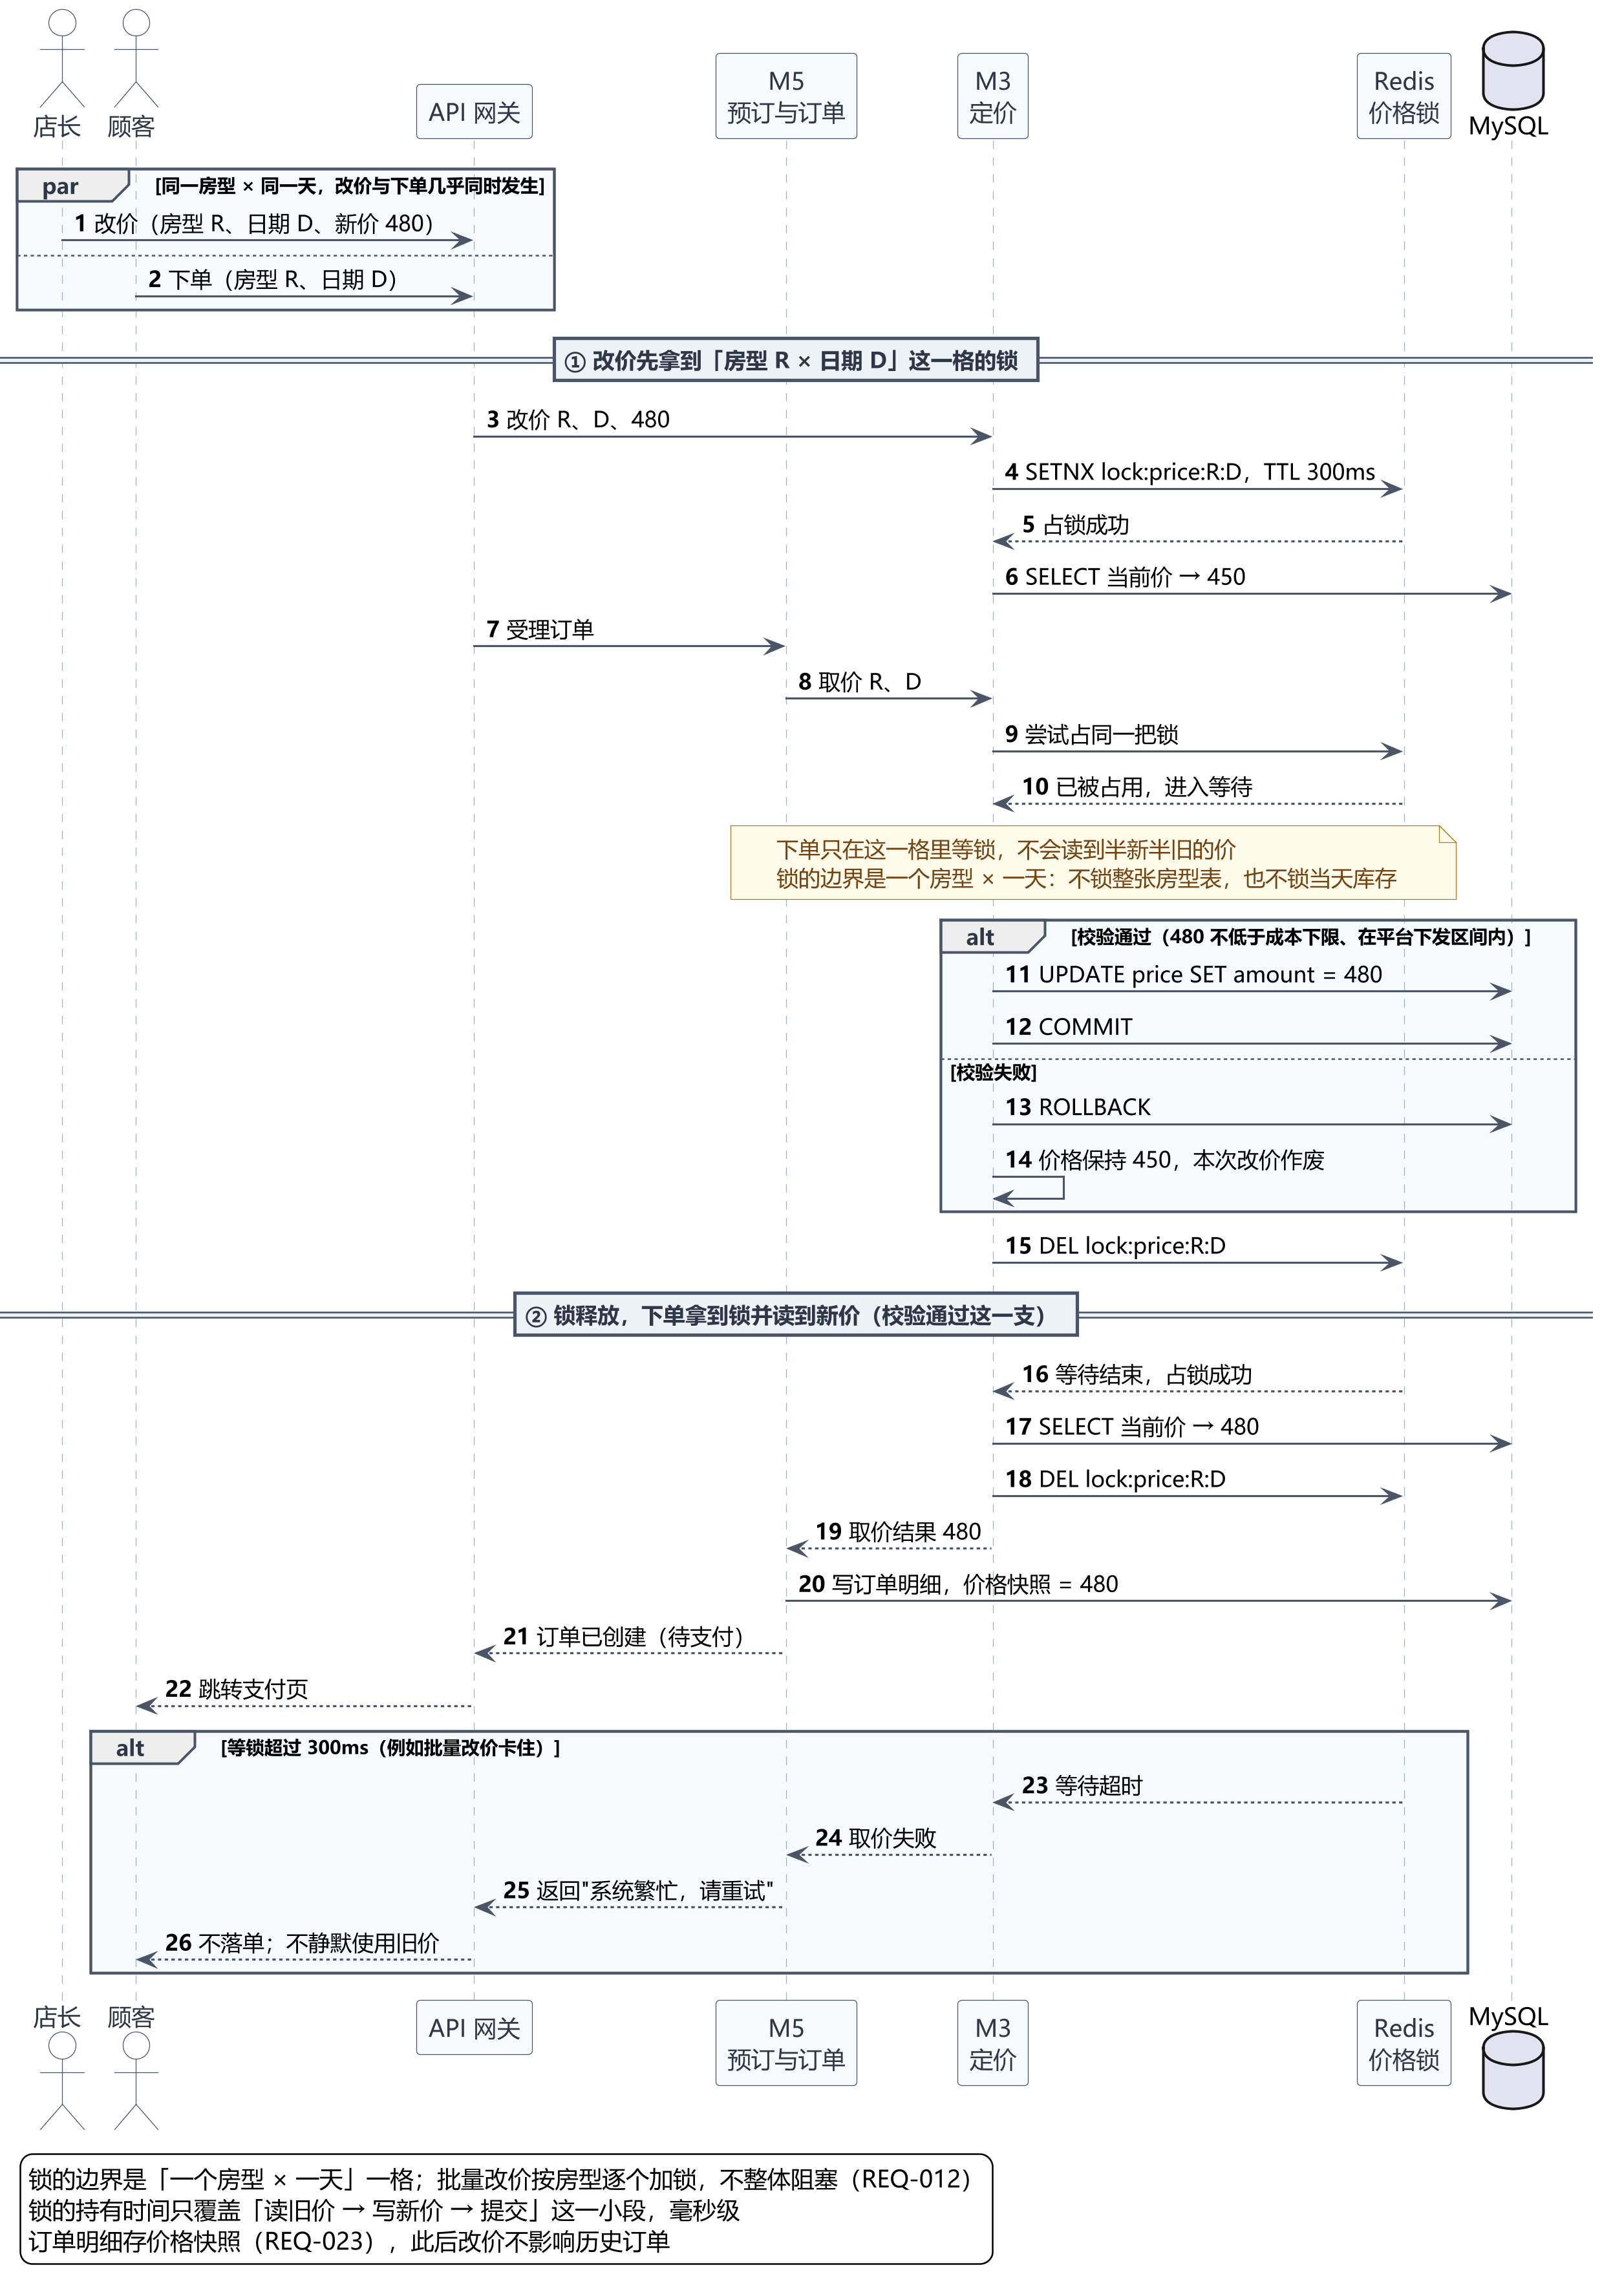
\includegraphics[width=0.68\textwidth]{../UML/UML时序图_改价互斥.png}
\caption{UML 时序图：改价与下单互斥}
\label{fig:seq2}
\end{figure}

改价互斥这张图最需要说明的是\textbf{锁的边界}。锁的粒度是「一个房型 $\times$ 一天」，不是整张房型表，也不是当天库存。批量改十个房型时按房型逐个加锁，不整体阻塞下单。锁的持有时间只覆盖「读旧价 $\rightarrow$ 写新价 $\rightarrow$ 提交」这一小段，毫秒级。

图的下半部分还有一条容易被忽略的分支：等锁超过 300 ms 时返回「系统繁忙，请重试」，订单不落库。这说明锁超时不是「降级使用旧价」，而是「明确告诉用户再来一次」。

\begin{figure}[htbp]
\centering
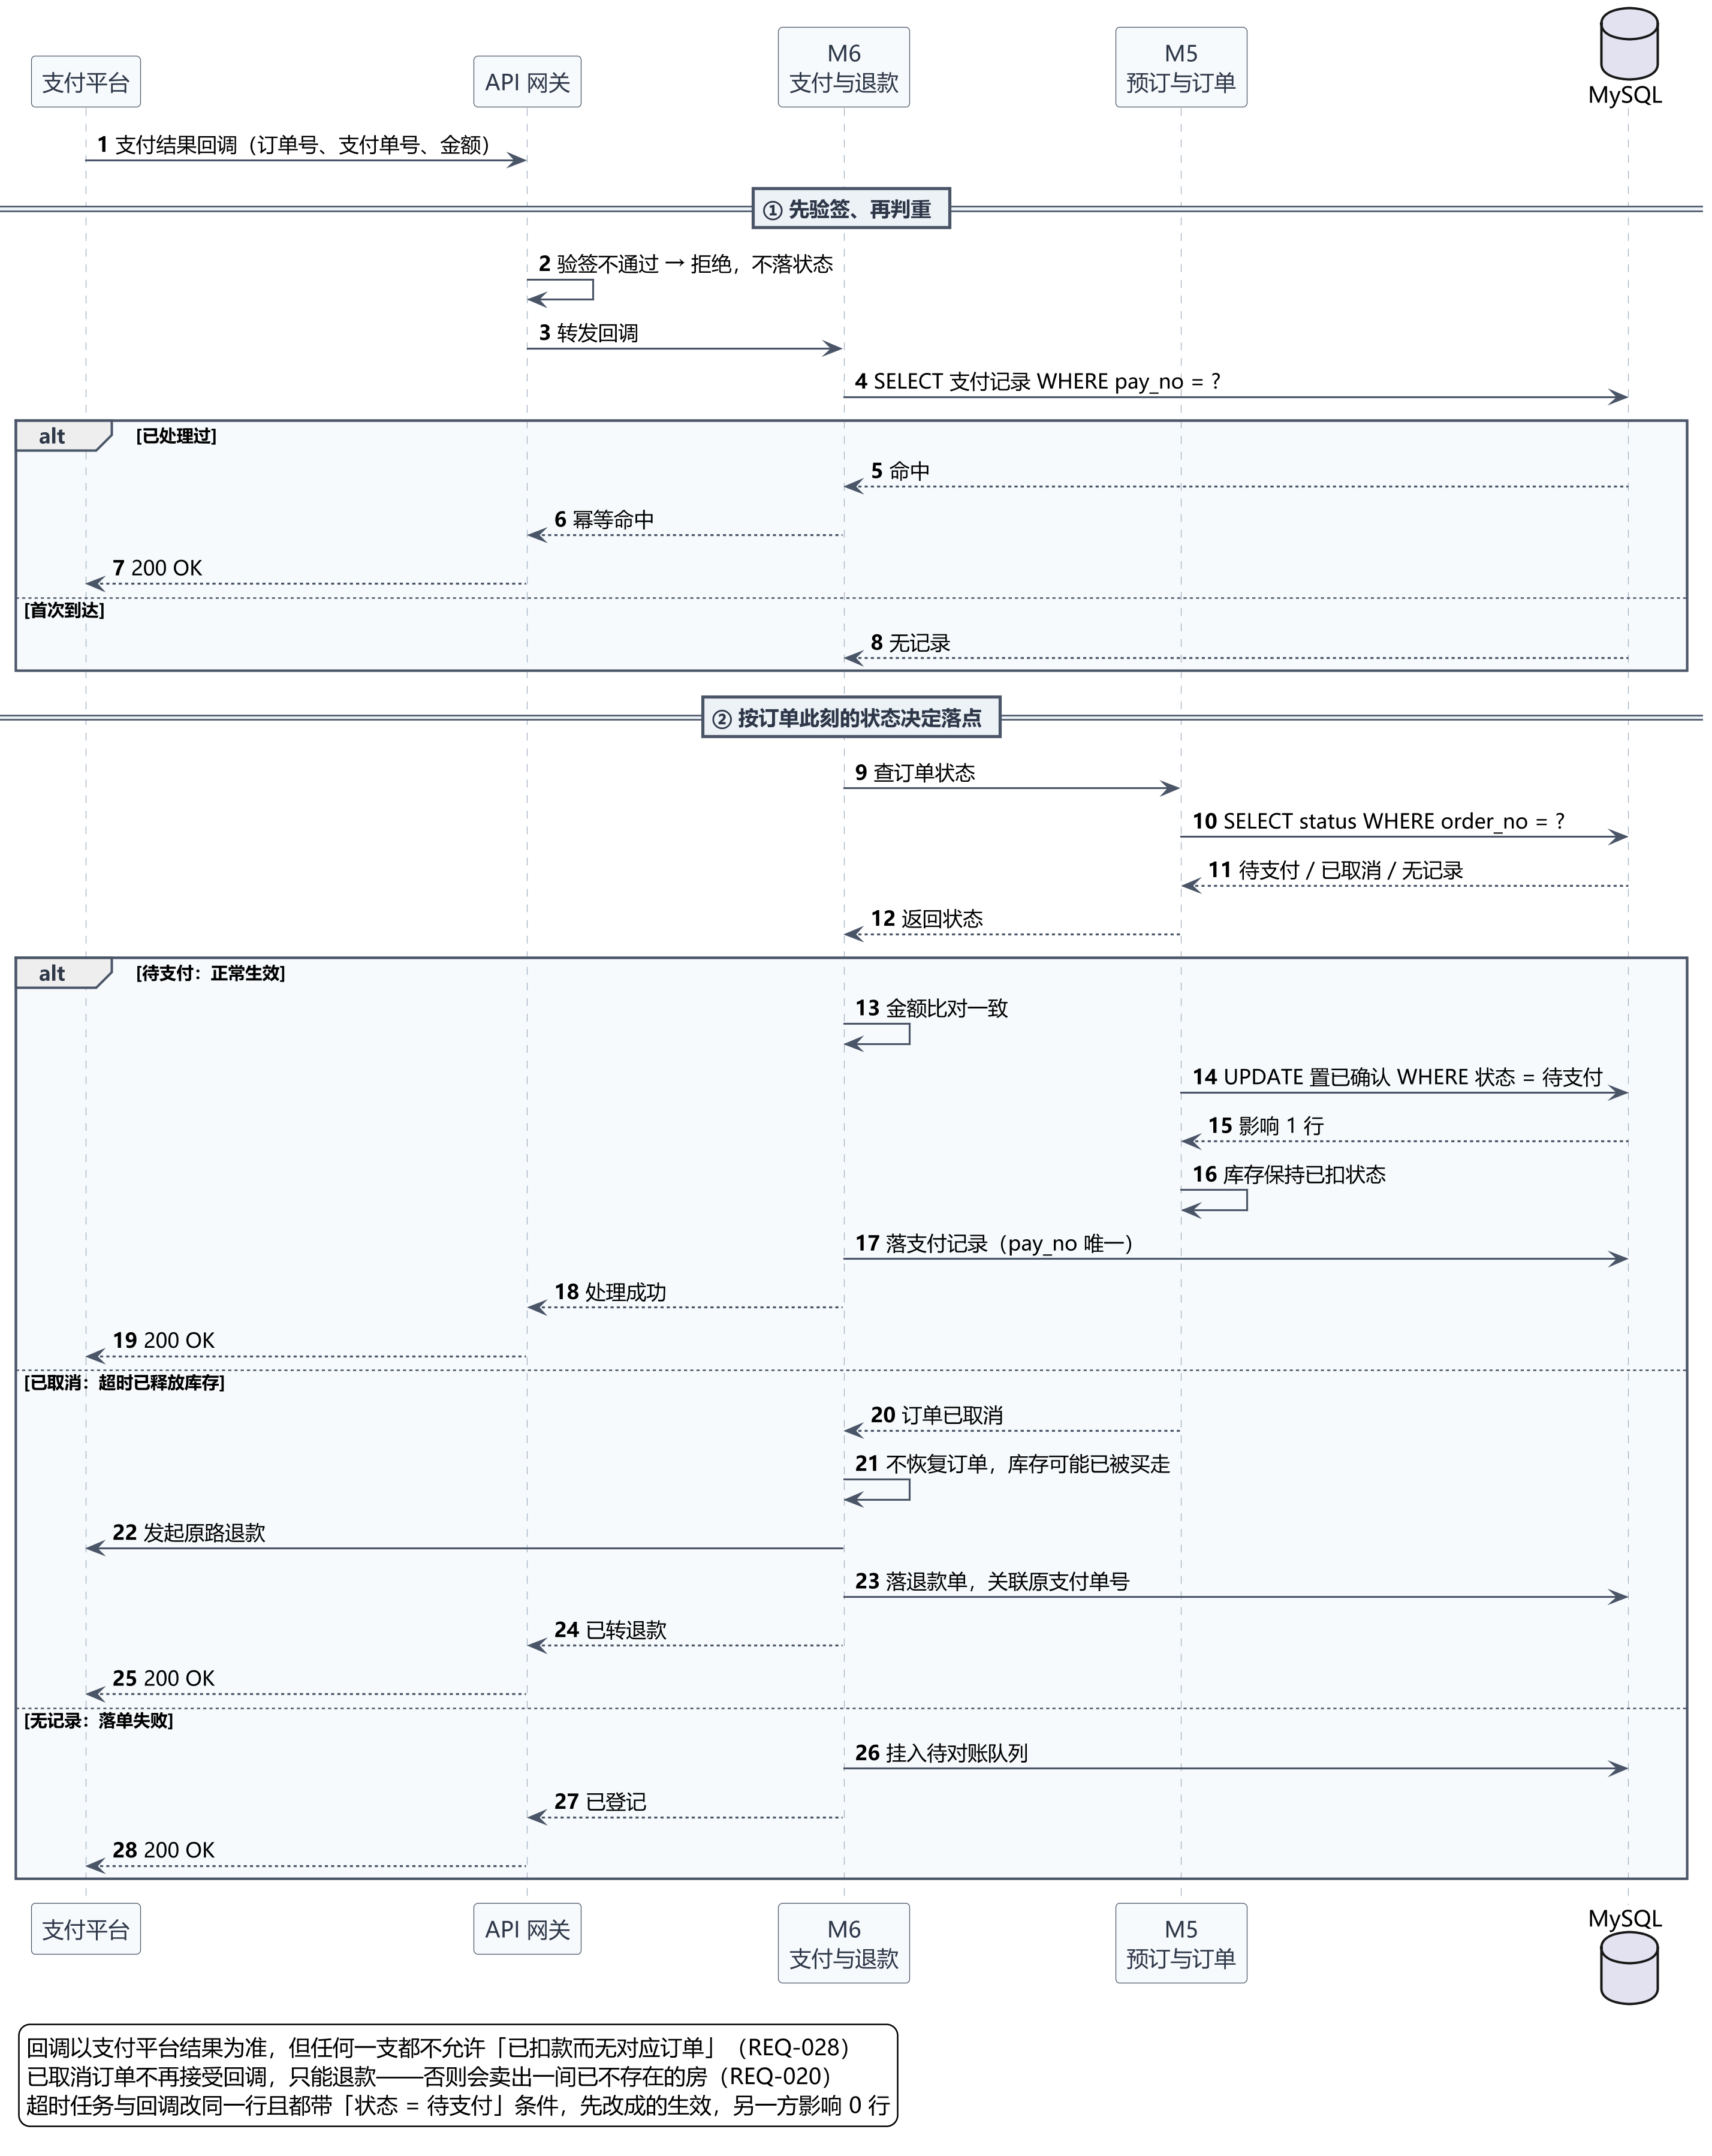
\includegraphics[width=0.77\textwidth]{../UML/UML时序图_支付回调.png}
\caption{UML 时序图：支付回调的三种落点}
\label{fig:seq3}
\end{figure}

支付回调这张图有一个 alt 三分支，分别对应订单此刻的三种状态：

\begin{itemize}
  \item \textbf{待支付}：正常生效，条件更新为已确认，落支付记录，库存保持已扣状态。
  \item \textbf{已取消}：说明超时任务先动手了，库存已经释放给别人。此时\textbf{不恢复订单}，改为原路退款——否则会卖出一间已经不存在的房。
  \item \textbf{无记录}：订单根本没建成功，挂入待对账队列，由每日对账补单或退款。
\end{itemize}

三种落点加起来，保证「已扣款而无对应订单」这个状态在任何时刻都不会停留超过一天。

\begin{figure}[htbp]
\centering
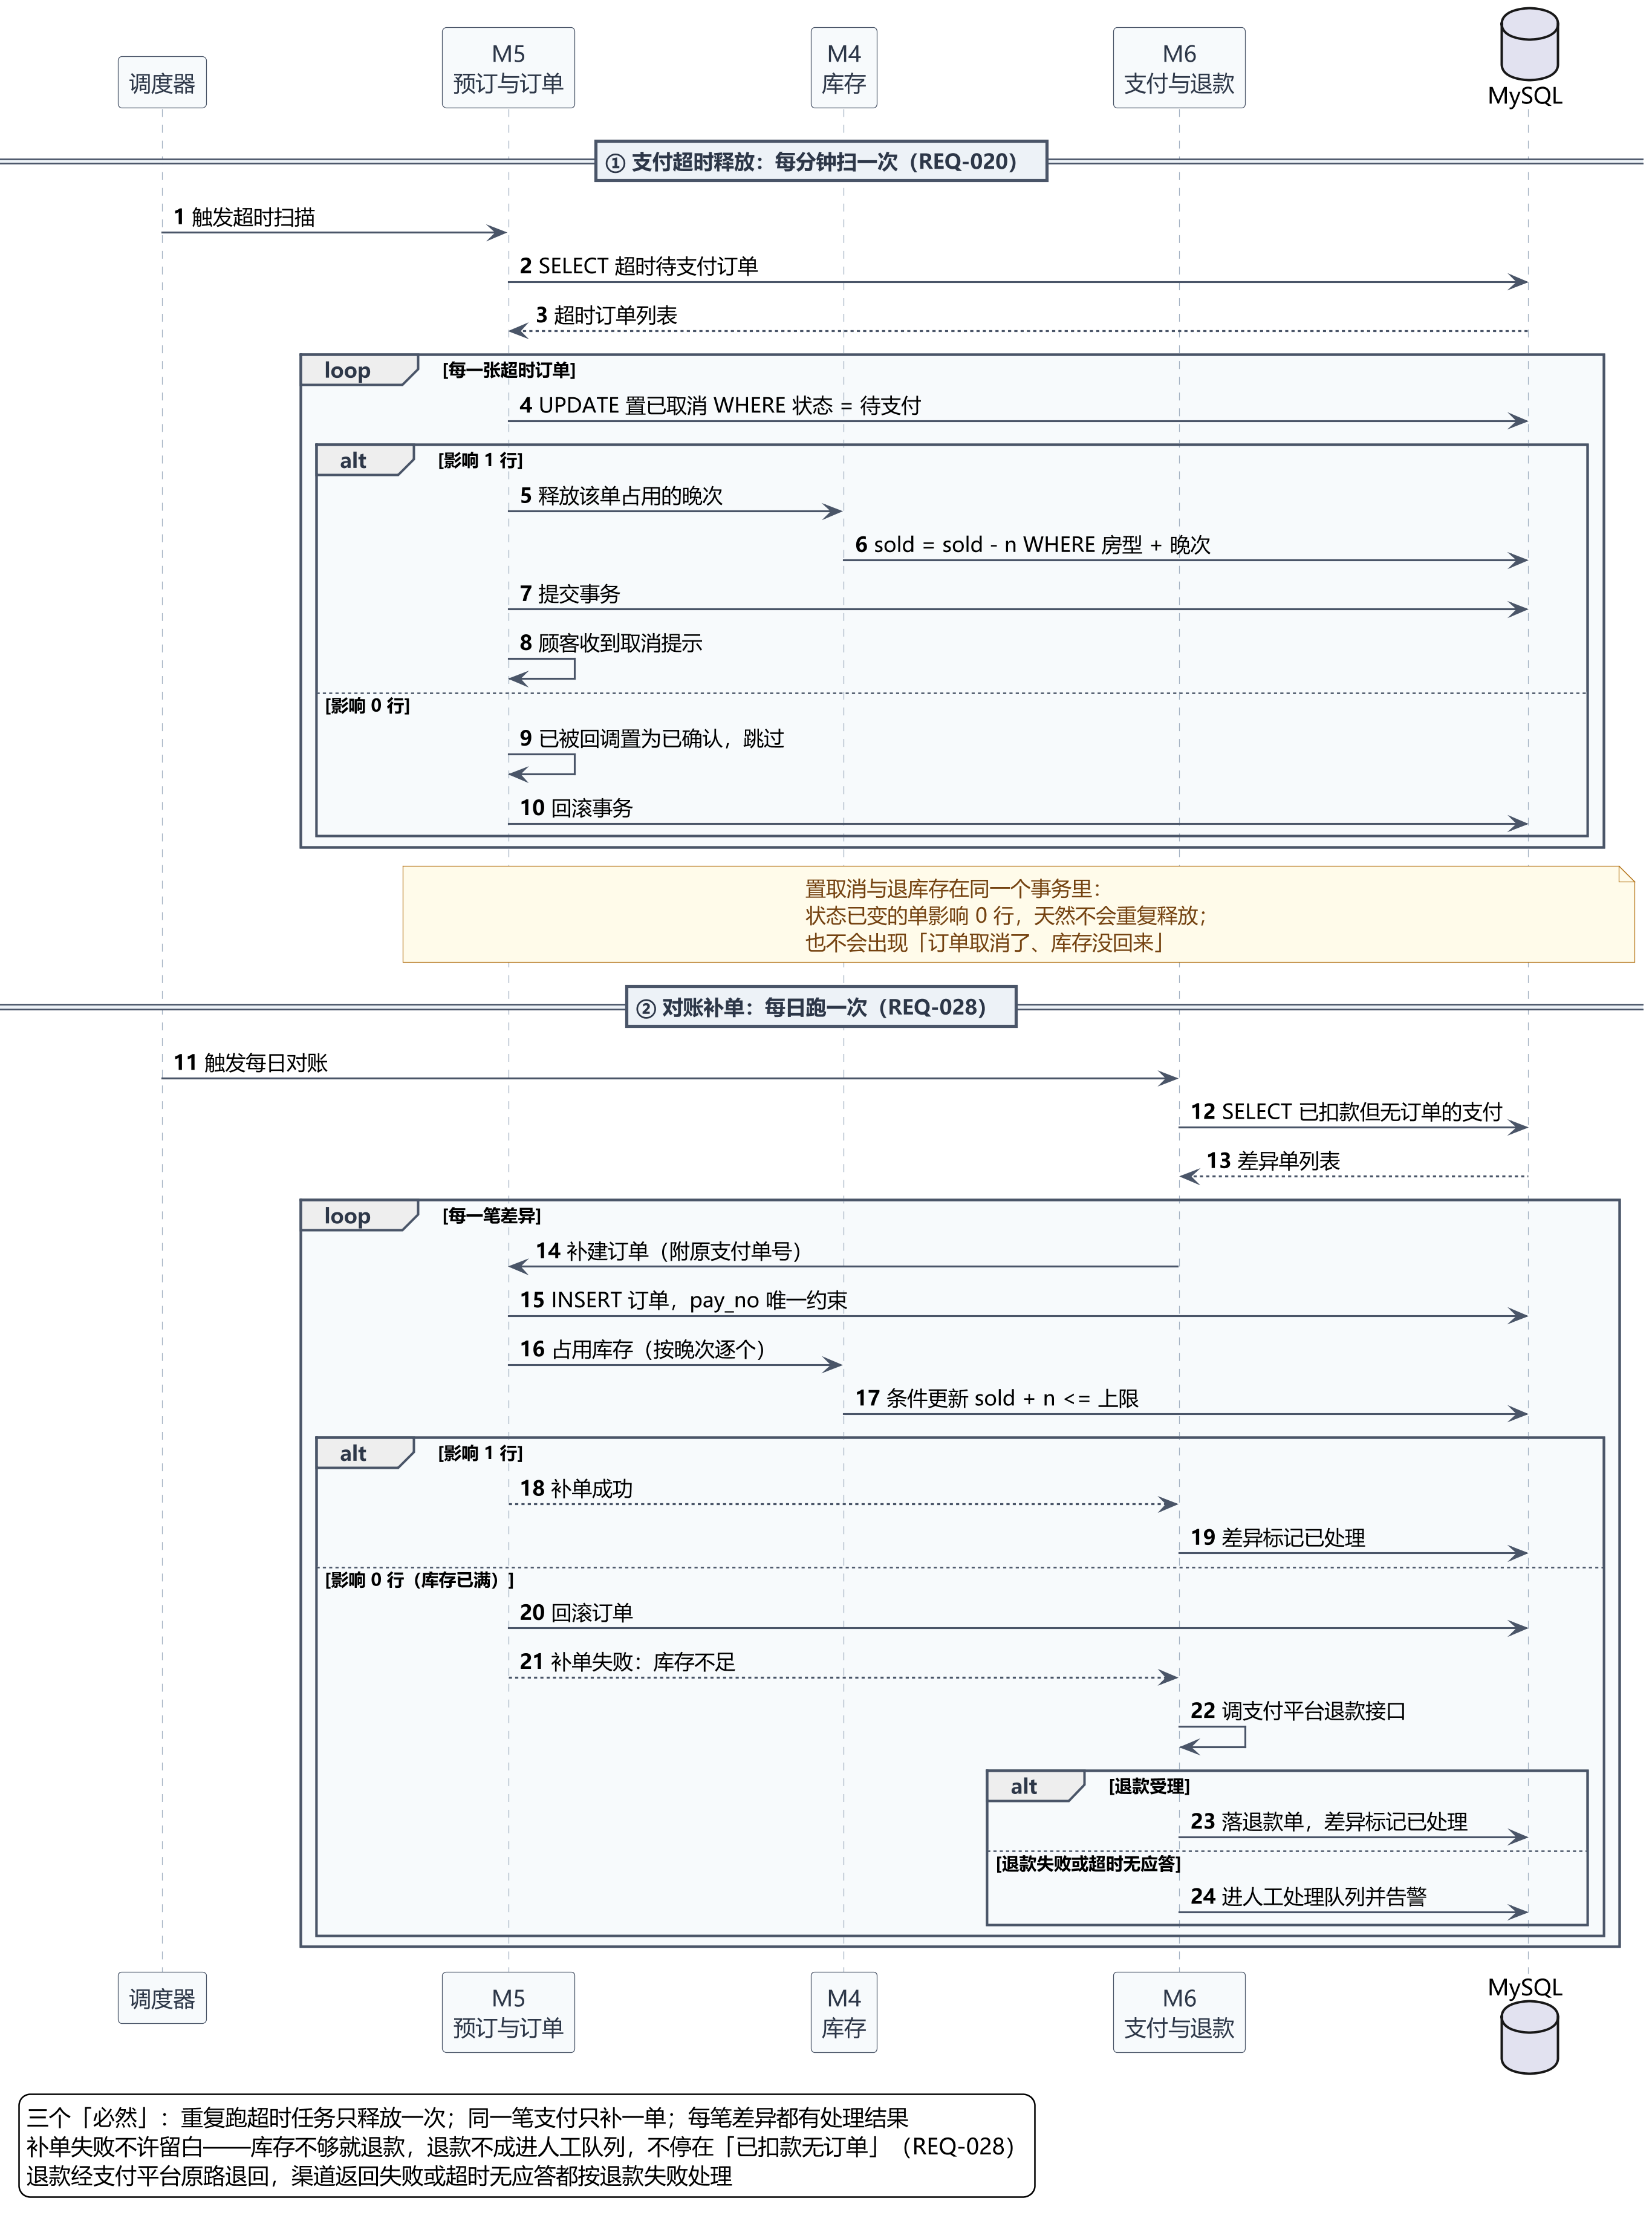
\includegraphics[width=0.72\textwidth]{../UML/UML时序图_超时释放与对账.png}
\caption{UML 时序图：超时释放与每日对账}
\label{fig:seq4}
\end{figure}

最后这张图有两条链路。上半部分是支付超时释放，每分钟扫描一次；关键在「置取消与退库存在同一个事务里」，并且置取消带「状态 = 待支付」条件——重复执行时影响 0 行，天然不会重复释放。

下半部分是对账补单，每日运行一次。补单逻辑里有一个必须写清的兜底：\textbf{库存不足时不是放弃，而是退款}。退款再失败就进人工队列并告警。这条兜底的意义是：对账的终点必须是「每笔差异都有处理结果」，不能停在「已扣款、无订单、待处理」。
